\documentclass{pracamgr}
\usepackage[a4paper,pdftex]{geometry}                                                                           % A4paper margins
\setlength{\oddsidemargin}{5mm}                                                                                         % Remove 'twosided' indentation
\setlength{\evensidemargin}{5mm}
\usepackage[protrusion=true,expansion=true]{microtype}  
\usepackage{amsmath,amsfonts,amsthm,amssymb}
\usepackage{graphicx}
\usepackage{parallel,enumitem}
\usepackage{amssymb}
\usepackage{float}
\usepackage{graphicx}
\usepackage{rotating}
\usepackage{amsmath, bm}
\usepackage{amsfonts}
\usepackage[T1]{fontenc}
\usepackage[polish,english]{babel}
\usepackage[utf8]{inputenc}
\usepackage{lmodern}
\usepackage{subfigure}
\usepackage{array}
\usepackage{etoolbox}
\usepackage{hyperref}
\usepackage{algorithm2e}
\usepackage[noend]{algpseudocode}
\usepackage{listings}
\usepackage[usenames,dvipsnames]{xcolor}
\usepackage{booktabs}
\usepackage{caption} 
\captionsetup[table]{skip=10pt}
\captionsetup[algorithm2e]{skip=10pt}
\usepackage{booktabs,caption,fixltx2e}
\usepackage[para,online,flushleft]{threeparttable}
\usepackage{adjustbox}
\usepackage{lscape}
\usepackage[round]{natbib}
\bibliographystyle{plainnat}
\usepackage{nameref}

\hypersetup{pdfstartview={XYZ null null 1.00}}

\hypersetup{
    colorlinks,
    linkcolor={red!50!black},
    citecolor={blue!50!black},
    urlcolor={blue!80!black}
}

\numberwithin{equation}{section}

\lstset{ %
  language=MATLAB,                     % the language of the code
  basicstyle=\footnotesize,       % the size of the fonts that are used for the code
  numbers=left,                   % where to put the line-numbers
  numberstyle=\tiny\color{gray},  % the style that is used for the line-numbers
  stepnumber=1,                   % the step between two line-numbers. If it's 1, each line
                                  % will be numbered
  numbersep=5pt,                  % how far the line-numbers are from the code
  backgroundcolor=\color{white},  % choose the background color. You must add \usepackage{color}
  showspaces=false,               % show spaces adding particular underscores
  showstringspaces=false,         % underline spaces within strings
  showtabs=false,                 % show tabs within strings adding particular underscores
  frame=single,                   % adds a frame around the code
  rulecolor=\color{black},        % if not set, the frame-color may be changed on line-breaks within not-black text (e.g. commens (green here))
  tabsize=2,                      % sets default tabsize to 2 spaces
  captionpos=b,                   % sets the caption-position to bottom
  breaklines=true,                % sets automatic line breaking
  breakatwhitespace=false,        % sets if automatic breaks should only happen at whitespace
  title=\lstname,                 % show the filename of files included with \lstinputlisting;
                                  % also try caption instead of title
  keywordstyle=\color{blue},      % keyword style
  commentstyle=\color{ForestGreen},   % comment style
  stringstyle=\color{Orchid},      % string literal style
  escapeinside={\%*}{*)},         % if you want to add a comment within your code
  morekeywords={*,...}            % if you want to add more keywords to the set
} 


\author{Michał Miktus}

\nralbumu{11716114}

\title{Machine learning approach \\
to DSGE estimation}

\kierunek{Analysis and Policy in Economics}

\opiekun{Pablo Winant Ph. D.\\
  Paris School of Economics\\
  }

\date{June 2019}

\newtheorem{theorem}{Theorem}
\newtheorem{corollary}{Corollary}[theorem]
\newtheorem{lemma}{Lemma}
\newtheorem{mydef}{Definition}

\begin{document}
\maketitle

 \begin{titlepage}
    
    \large
    \null
    \vfill
    
  \textbf{\Large Declaration of the supervisor} 
      \vspace{3mm}
      
   I declare the following thesis project was written under my supervision and I state that the project meets all submission criteria for the procedure of academic degree award.\\
   \vspace{5mm}
   
   Date \hfill Signature of the Supervisor
   
   \vspace{2cm}
   \textbf{\Large Declaration of the author of the project}
    \vspace{3mm}
    
   Aware of legal responsibility, I declare that I am the sole author of the following thesis project and that the project I submit is entirely free from any content that constitutes copyright infringement or has been acquired contrary to applicable laws and regulations.\\
   
   I also declare that the below project has never been subject of degree-awarding procedures in any school of higher education.\\

   Moreover I declare that the attached version of the thesis project is identical with the enclosed electronic version.\\
   \vspace{5mm}
   
   Date  \hfill Signature of the Author 
    \vspace{3cm}
 
\end{titlepage}
    
\begin{abstract}
Here goes the abstract. \\
\end{abstract}

\tableofcontents
\listoffigures
\listoftables
\listofalgorithms


\chapter*{Introduction} \label{Introduction}
\addcontentsline{toc}{chapter}{Introduction}

Here goes the introduction. \\

\chapter{Dynamic Stochastic General Equilibrium (DSGE) model} \label{Dynamic Stochastic General Equilibrium (DSGE) model}

It is generally acknowledged that a satisfactory macroeconomic model should be grounded on rational intertemporal optimizing behavior of microagents, satisfying the rational expectations assumption. Furthermore, it should reflect the imperfectly flexible wages and prices, associated with deficiencies on labor and product markets. One of the most renowned New Keynesian model satisfying the above-mentioned presumptions was developed by \citet{smets2003estimated}, as the elaboration of previous work of \citet{christiano2005nominal}.

Succinctly, it assumes that in the closed economy framework there exists a continuum of households, who supply household-specific labor in monopolistically competitive environment. In addition, they set Calvo-sticky wages, deriving utility from consumption relative to their habits and disutility from work. Households save and part of their savings is transformed into capital through a household technology, which in turn has its own adjustment costs. Moreover, they rent out their capital to the intermediate-good sector and choose total amount of  investment with variable capital utilization rate. The rest of their savings is spent for lending and borrowing decisions, not to mention the bond holding settlements.

On the firm side, a continuum of intermediate goods produced by firms in monopolistic competition is assumed. Their production requires various kinds of differentiated labor and (homogeneous) capital, leading to the Calvo-sticky prices setting. On the other hand, final goods are produced in perfect competition framework through intermediate goods and they are consumed by households and government, allowing for the fiscal policy and Taylor-type monetary policy rule.

Finally, there is a plethora of sources of shocks, such as two preference shocks, labor substitutability shock, intermediate-goods substitutability shock and aggregate productivity shock, goods mark-up or cost push shock, shocks to investment cost or monetary policy rule shock (similarly to the \citet{christiano2005nominal}).

After introduction of the main essence of the \citet{smets2003estimated}  model, in the following sections it will be derived meticulously.

\section{Households} \label{DSGE - Households}

In the examined economy, there is a continuum of mass one households indexed by $\tau \in (0,1)$, maximizing an intertemporal utility function over an endless horizon:

\begin{equation}
 \mathbb{E}_{0} \left(\sum\limits_{t=0}^{\infty} \beta^{t} U_{t}^{\tau} \right) 
\end{equation}

where $\beta$ is the discount factor and $U_{t}^{\tau}$ stands for the contemporaneous utility
function depending on consumption $C_{t}^{\tau}$, and labor $l_{t}^{\tau}$.

The utility function is separable in its two arguments:

\begin{equation}
U_{t}^{\tau} \left( C_{t}^{\tau}, l_{t}^{\tau} \right) = \varepsilon^{B}_{t} \left[ \frac{1}{1-\sigma_{c}} \left( C_{t}^{\tau} - H_{t} \right)^{1-\sigma_{c}} - \frac{\varepsilon_{t}^{L}}{1+\sigma_{l}} \left( l_{t}^{\tau} \right)^{1+\sigma_{l}} \right]
\end{equation}

where $\sigma_{c}$ is the measure of relative risk aversion or the inverse of the intertemporal elasticity of substitution, while $\frac{1}{\sigma_{l}}$ denotes the elasticity of labor with respect to the real wage.

The above-mentioned utility function includes two shocks, namely a general preference shock $\varepsilon^{B}_{t}$ affecting intertemporal substitution of households and a labor supply shock $\varepsilon^{L}_{t}$. All of them follow autoregressive processes of the first order with normally and independently distributed error terms:

\begin{align}
& \varepsilon^{B}_{t} = \rho_{B} \cdot \varepsilon^{B}_{t-1}+ \eta_{t}^{B}, \enspace \enspace \eta_{t}^{B} \sim \mathcal{N}(0,1) \\
& \varepsilon^{L}_{t} = \rho_{L} \cdot \varepsilon^{L}_{t-1}+ \eta_{t}^{L}, \enspace \enspace\enspace \eta_{t}^{L} \sim \mathcal{N}(0,1) 
\end{align}

The utility function includes as well a habit $H_{t}$ that is proportional to the aggregate past consumption:

\begin{equation}
H_{t} = h \cdot C_{t-1}
\end{equation}

which allows the optimal behavior of households to respond to shocks with an hump-shaped and lagged path of the optimal consumption. It has to be underlined that the habit variable depends on lagged aggregate consumption that is unaffected by any one agent's decisions.

Furthermore, the income of the households $Y_{t}^{\tau}$ takes the form of:

\begin{equation}
Y_{t}^{\tau} = \frac{W_{t}^{\tau}}{P_{t}} \cdot l_{t}^{\tau} + A_{t}^{\tau} + D_{t}^{\tau} + \left( r_{t}^{k} z_{t}^{\tau} - \Psi(z_{t}^{\tau}) \right) K_{t-1}^{\tau} - T_{t}
\end{equation}

thus depending on real labor income $l_{t}^{\tau} \cdot \frac{W_{t}^{\tau}}{P_{t}} $, net cash inflow from participating in state-contingent securities $A_{t}^{\tau}$, the dividends derived from the imperfect competitive intermediate firms $D_{t}^{\tau}$, taxes $T_{t}$ and the return on the real capital stock depreciated by the cost associated with variations in the degree of capital utilization $z_{t}^{\tau}$. It is assumed that the cost of capital utilization is zero when capital utilization is one ($\Psi(1) = 0$) as it would in the steady state. Framing differently, households rent capital services to firms and decide about the amount of capital to accumulate given certain capital adjustment costs. With the augmentation of the rental price of capital, the capital stock can be used more intensively according to a specific cost schedule.

Households hold their financial wealth in the form of bonds $B_{t}$, which are one-period securities with market price $b_{t}$ and gross return:

\begin{equation}
R_{t} = 1 + i_{t}= \frac{1}{b_{t}}
\end{equation}

Current income and financial wealth can be used for consumption and investment in physical capital, thus households maximize their objective function subject to an intertemporal budget constraint:

\begin{equation}
C_{t}^{\tau} + I_{t}^{\tau} + b_{t} \frac{B_{t}^{\tau}}{P_{t}} = Y_{t}^{\tau} + \frac{B_{t-1}^{\tau}}{P_{t}}
\end{equation}

Finally, following \citet{christiano2005nominal}, it is assumed that there exist state-contingent securities that perfectly insure the households against variations in household specific labor income. As a result, the labor income plus the net cash-inflow from participating in state-contingent securities component $\frac{W_{t}^{\tau}}{P_{t}} \cdot l_{t}^{\tau} + A_{t}^{\tau}$ in the household's income will be equal to aggregate labor income. Analogously the consumption of an individual household will equal the aggregate consumption and the marginal utility of consumption will be identical across different types of households. Consequence, capital holdings $K_{t}^{\tau} \equiv K_{t}$, bond holdings $B_{t}^{\tau} \equiv B_{t}$ as well as firm dividends  $D_{t}^{\tau} \equiv D_{t}$ will be indistinguishable across different types of households.

\subsection{Consumption and savings behavior} \label{Consumption and savings behavior}

The maximization of the objective function of the household subject to the budget constraint with respect to consumption and holdings of bonds, may be performed through the Lagrangian-based technique, yielding the first-order condition for consumption growth in the existence of external habit formation:

\begin{align}
\mathbb{E}_{t} \left[ \beta \frac{\varepsilon_{t+1}^{B} (C_{t+1}^{\tau} - h \cdot C_{t} )^{-\sigma_{c}}}{\varepsilon_{t}^{B} (C_{t}^{\tau} - h \cdot C_{t-1} )^{-\sigma_{c}}} R_{t} \frac{P_{t}}{P_{t+1}} \right] = 1
\end{align}

or equivalently:

\begin{align}
\mathbb{E}_{t} \left[ \beta \frac{\lambda_{t+1}}{\lambda_{t}} R_{t} \frac{P_{t}}{P_{t+1}} \right] = 1
\end{align}

where:

\begin{align}
\lambda_{t} = \frac{\partial U_{t}^{\tau}}{\partial C_{t}^{\tau}} = \varepsilon_{t}^{B} (C_{t}^{\tau} - H_{t} )^{-\sigma_{c}} = \varepsilon_{t}^{B} (C_{t}^{\tau} - h \cdot C_{t-1} )^{-\sigma_{c}} = \varepsilon_{t}^{B} (C_{t} - h \cdot C_{t-1} )^{-\sigma_{c}}
\end{align}

The exact calculations for the whole chapter's derivations are performed in the \nameref{Appendix A}.

\subsection{Labor supply decisions and the wage setting equation} \label{Labor Supply decisions and the wage setting equation}

Households differ, supply ing a differentiated type of labor. Thus, each household has a monopoly power over the supply of its labor. In other words, labor is a differentiated good, supplied by households in a monopolistic competition to the production sector. Consequently, firms consider labor supplies $l_{t}^{\tau}$ as imperfect substitutes. The aggregate labor demand $L_{t}$ and the aggregate nominal wage $W_{t}$ are given by the following Dixit-Stiglitz type aggregator, where $\lambda_{w ,t} > 0$ is the substitution parameter:

\begin{align}
L_{t} &= \left[ \int\limits_{0}^{1} \left( l_{t}^{\tau} \right)^{\frac{1}{1+\lambda_{w,t}}} d\tau \right]^{1+\lambda_{w,t}}
\end{align}

It can be observed that the condition $\lambda_{w ,t} = 0$ would correspond to the perfect substitution of labor.

Therefore, firms minimize the cost function $\int\limits_{0}^{1} W_{t}^{\tau} l_{t}^{\tau} d\tau$ under the aggregate labor demand, which in turn yields:

\begin{align} \label{Aggregate labor demand}
L_{t} &= \left[ \int\limits_{0}^{1} \left( \frac{W_{t}^{\tau}}{W_{t}}\right)^{\frac{-1}{\lambda_{w ,t}}} L_{t}^{\frac{1}{1+\lambda_{w ,t}}} d\tau \right]^{1+\lambda_{w,t}} \nonumber \\
& \iff W_{t} = \left[ \int\limits_{0}^{1} \left( W_{t}^{\tau} \right)^{\frac{-1}{\lambda_{w ,t}}}  d\tau \right]^{-\lambda_{w,t}}
\end{align}

where the Lagrange multiplier $W_{t}$ can be interpreted as well as the price of a working hour and thus a wage index.

In addition, the determination of wages follows a Calvo rule. In other words, each household $\tau$ has a (constant) probability of $1-\varsigma_{w}$ in every period $t$ to be able to set its nominal wage and therefore in each period $t$ a fraction of $1-\varsigma_{w}$ households adapts its wage. Moreover, wages of the fraction of households $\varsigma_{w}$ that cannot reoptimize are partially anchored to the inflation rate:

\begin{align}
W_{t}^{\tau} = \left( \Pi_{t-1} \right)^{\gamma_{w}}W_{t-1}^{\tau} = \left( \frac{P_{t-1}}{P_{t-2}} \right)^{\gamma_{w}}W_{t-1}^{\tau}
\end{align}

where $\gamma_{w}$ is the degree of wage indexation, such that $\gamma_{w} = 0$ entails no indexation ($W_{t}^{\tau} = W_{t-1}^{\tau}$), while $\gamma_{w} = 1$ suggests a complete indexation ($W_{t}^{\tau} = \Pi_{t-1} W_{t-1}^{\tau}$).

After denoting by $\widetilde{W}_{t}$ the wage of the household that in period t can reoptimize, it follows:

\begin{align}
W_{t}^{\tau} = \begin{cases}
\widetilde{W}_{t} & \text{with probability} \enspace 1-\varsigma_{w} \\
\left( \Pi_{t-1} \right)^{\gamma_{w}}W_{t-1}^{\tau} & \text{with probability} \enspace \varsigma_{w} 
\end{cases}
\end{align}

The equation of motion for the aggregate wage index $W_{t}$ can be obtained through \ref{Aggregate labor demand}:

\begin{align}
\left(W_{t}\right)^{\frac{-1}{\lambda_{w,t}}} &= \varsigma_{w} \cdot \int\limits_{0}^{1} \left( W_{t-1}\left( \frac{P_{t-1}}{P_{t-2}} \right)^{\gamma_{w}} \right)^{\frac{-1}{\lambda_{w,t}}} d\tau + (1 - \varsigma_{w}) \cdot \int\limits_{0}^{1} \widetilde{W}_{t}^{\frac{-1}{\lambda_{w,t}}} d\tau = \nonumber \\ 
& = \varsigma_{w}\cdot \left[ W_{t-1}\left( \frac{P_{t-1}}{P_{t-2}} \right)^{\gamma_{w}} \right]^{\frac{-1}{\lambda_{w,t}}} + (1 - \varsigma_{w}) \cdot \widetilde{W}_{t}^{\frac{-1}{\lambda_{w,t}}}
\end{align}

The probability for $\widetilde{W}_{t}$ not to re-set until period $i$ is $\left( \varsigma_{w} \right)^{i}$, thus through the indexation the not reoptimized wage in period $t+i$ becomes:

\begin{align}
W_{t}^{\tau} &= \widetilde{W}_{t} \nonumber \\
W_{t+1}^{\tau} &= \left( \frac{P_{t}}{P_{t-1}} \right)^{\gamma_{w}} W_{t}^{\tau} = \left( \frac{P_{t}}{P_{t-1}} \right)^{\gamma_{w}} \widetilde{W}_{t}  \nonumber \\
W_{t+2}^{\tau} &= \left( \frac{P_{t+1}}{P_{t}} \right)^{\gamma_{w}}  W_{t+1}^{\tau} = \left( \frac{P_{t+1}}{P_{t}} \right)^{\gamma_{w}} \left( \frac{P_{t}}{P_{t-1}} \right)^{\gamma_{w}}  W_{t}^{\tau}  = \left( \frac{P_{t+1}}{P_{t-1}} \right)^{\gamma_{w}} \widetilde{W}_{t} \nonumber \\ \vdots \nonumber \\
W_{t+i}^{\tau} &= \left( \frac{P_{t+i-1}}{P_{t-1}} \right)^{\gamma_{w}} \widetilde{W}_{t} \nonumber \\
\end{align}

Households that can re-set their wages maximize their objective function subject to their budget constraint and the demand of labor, taking into consideration the fact that wages remain fixed until period $i$ with a probability $\left( \varsigma_{w} \right)^{i}$, which yields:

\begin{align}
\frac{\widetilde{W}_{t}}{P_{t}} &\mathbb{E}_{t} \left\{ \sum\limits_{i=0}^{\infty} \beta^{i} \varsigma_{w}^{i} \left( \frac{P_{t+i-1}}{P_{t-1}} \right)^{\gamma_{w}}  \frac{P_{t}}{P_{t+i}} \left( \frac{l_{t+1}^{\tau} U_{t+i}^{C}}{1 + \lambda_{w, t+i}} \right) \right\} = \nonumber \\
&= \mathbb{E}_{t} 
\left\{ \sum\limits_{i=0}^{\infty} \beta^{i} \varsigma_{w}^{i} l_{t+1}^{\tau} U_{t+i}^{l} \right\}
\end{align}

Assuming perfect flexibility of wages $(\varsigma_{w} = 0)$, the above-mentioned equation becomes:

\begin{align}
\frac{\widetilde{W}_{t}}{P_{t}} = \left(1 + \lambda_{w, t} \right)\frac{U_{t}^{L}}{U_{t}^{C}}
\end{align}

It will be moreover assumed that the degree of substitutability $\lambda_{w, t}$ is affected by a normally and independently distributed shocks:

\begin{align}
\lambda_{w, t} = \lambda_{w} + \eta_{t}^{w}, \quad \eta_{t}^{w} \sim \mathcal{N} \left(0, \sigma^{2}_{\eta_{w}} \right)
\end{align}

In the flexible-wage economy, $1+\lambda_{w, t}$ will be the markup of real wages over the usual ratio of the marginal disutility of labor to the marginal utility of consumption. Thus, $\eta_{t}^{w}$ can be regarded as a wage markup shock.

\subsection{Capital accumulation and investment decision} \label{Capital accumulation and investment decision}

Households own the stock of capital of the economy and rent it at the rate $r_{t}^{k}$ to the firms of the intermediate sector. Moreover, investment in period $t-1$ increases the stock of capital in period $t$ and households are assumed to choose the utilization rate $z_{t}$ of their stock of capital. The equation of motion of capital becomes:

\begin{align}
K_{t} = K_{t-1} (1 - \tau) + I_{t} \left[ 1 - S \left(\frac{\varepsilon_{t}^{I}I_{t}}{I_{t-1}} \right) \right]
\end{align}

where $\tau$ is the depreciation rate, while the function $S$ introduces in the model the adjustment costs for investment that depend on its rate of growth, proposed in order to avoid strong oscillations of capital. It will be  furthermore assumed that for the constant growth rate of investment, as in the steady state, $S(1)=0$ and similarly in the neighborhood of the steady state $S'(1) = 0$. Hence, adjustment costs depend only on the second derivative such that $S''(1)>0$. Finally, the function $S$ is subject to a shock $\varepsilon_{t}^{I}$ following an $AR(1)$ process:

\begin{align}
\varepsilon_{t}^{I} = \rho_{I} \varepsilon_{t-1}^{I} + \eta_{t}^{I}, \quad  \eta_{t}^{I} \sim \mathcal{N} \left(0,1\right)
\end{align}

Solving the respective maximization problem with the Lagrange multiplier in the form of $\lambda_{t} Q_{t}$ yields:

\begin{align}
&r_{t}^{k} = \Psi'(z_{t})  \\
&Q_{t} = \mathbb{E}_{t} \left[ \beta \frac{\lambda_{t+1}}{\lambda_{t}} \left( Q_{t+1}(1-\tau) + z_{t+1}r_{t+1}^{k} - \Psi(z_{t+1}) \right) \right]  \\
&\mathbb{E}_{t} \left[ -\beta^{t} \lambda_{t} - \beta^{t} \lambda_{t} Q_{t} \left(-1 + S\left(\frac{\varepsilon_{t}^{I}I_{t}}{I_{t-1}} \right) + I_{t} \cdot S' \left(\frac{\varepsilon_{t}^{I}I_{t}}{I_{t-1}} \right) \cdot \frac{\varepsilon_{t}^{I}}{I_{t-1}} \right) \right] = \nonumber \\
\qquad &= \mathbb{E}_{t} \left[ \beta^{t+1} \lambda_{t+1} Q_{t+1} \left(I_{t+1} \cdot S' \left(\frac{\varepsilon_{t+1}^{I}I_{t+1}}{I_{t}} \right) \cdot \frac{-\varepsilon_{t+1}^{I} I_{t+1}}{I_{t}^{2}} \right) \right]
\end{align}

In other words the capital utilization rate is set so that the revenue $r_{t}^{k}$ of the marginal utilization equals the marginal costs $\Psi'(z_{t})$, the real value of the stock of capital today $\lambda_{t} Q_{t}$ is equal to the expected value of sum of not depreciated stock of capital of the next period $\lambda_{t+1}Q_{t+1}(1-\tau)$ and the expected revenue of the future utilization $ z_{t+1}r_{t+1}^{k}$ minus the related costs $\Psi(z_{t+1})$, while the costs of the marginal investment (included the adjustment costs) must be equal to the expected marginal revenue of investment.

In addition, $\lambda_{t} Q_{t}$ can be viewed as the marginal value of capital. Therefore, regarding the fact that $\lambda_{t}$ equals the marginal utility of consumption, $Q_{t}$ can be interpreted as marginal Tobin-Q (the ratio of the marginal value of capital due to the increase of the capital stock over the marginal opportunity cost):

\begin{align}
Q_{t} = \frac{\lambda_{t} Q_{t}}{\lambda_{t}}
\end{align}

At the steady-state $Q=1$, thus marginal revenues and costs compensate each other. If $Q>1$ there are incentives to increase the capital accumulation through investment, while if $Q<1$ the reverse holds true.

\section{Firms} \label{DSGE - Firms}

The economy produces only one final product $Y_{t}$ and a continuum of intermediates goods defined over $j \in [0,1]$, such that firm $j$ produces the intermediate product $y_{t}^{j}$ . Firms of the final product sector operate in a (perfect) competitive market, while firms in the intermediate sector function in a monopolistic competition and set their prices forward-looking.

\subsection{Final product sector} \label{DSGE - Firms- Final product sector}

For the production of the final product $Y_{t}$ firm use the intermediate products $y_{t}^{j}$ as input, with aggregation performed through the following technology:

\begin{align} \label{Technology constraint}
Y_{t} = \left[ \int\limits_{0}^{1} \left(y_{t}^{j} \right)^\frac{1}{1+\lambda_{p,t}} dj \right]^{1+\lambda_{p,t}}
\end{align}

Define $p_{t}^{j}$ as the price of the intermediate product $y_{t}^{j}$ , then the representative firm minimizes the cost function $\int\limits_{0}^{1} p_{t}^{j} y_{t}^{j}dj$ of a particular combination of inputs observing the constraint \ref{Technology constraint}. Solving the minimization problem through Lagrangian, with $P_{t}$ as the Lagrange multiplier, yields:

\begin{align} \label{Optimal prices for firm}
Y_{t} &=  \left[ \int\limits_{0}^{1} \left( \frac{ p_{t}^{j}}{P_{t}} \right)^{\frac{-1}{\lambda_{p,t}}} Y_{t}^\frac{1}{1+\lambda_{p,t}} dj \right]^{1+\lambda_{p,t}} \nonumber \\
& \iff P_{t} = \left[ \int\limits_{0}^{1} \left( p_{t}^{j} \right)^{\frac{-1}{\lambda_{p,t}}} dj \right]^{-\lambda_{p,t}}
\end{align}

where $P_{t}$ can be interpreted as the price index of the final good sector, while $\lambda_{p,t}$ is a stochastic parameter representing the mark-up of the good market (or a cost-push shock), such that:

\begin{align}
\lambda_{p,t} = \lambda_{p} + \eta_{t}^{p}, \quad \eta_{t}^{p} \sim \mathcal{N} \left(0, \sigma^{2}_{\eta_{t}^{p}} \right)
\end{align}

\subsection{Intermediate product sector} \label{DSGE - Firms - Intermediate product sector}

Each firm $j$ of the intermediate good sector minimizes its labour and capital costs $W_{t}L_{j,t} + r_{t}^{k} \widetilde{K}_{j,t}$, observing its Cobb-Douglas production function:

\begin{align}
y_{t}^{j} = \varepsilon_{t}^{a} \widetilde{K}_{j,t}^{\alpha} L_{j,t}^{1-\alpha} - \Phi
\end{align}

where $\widetilde{K}_{j,t}$ is the effective utilized stock of capital given by $\widetilde{K}_{j,t} = z_{t}K_{j,t-1}$, $L_{j,t}$ is the index of the differently utilized labour force, while $\Phi$ are the fixed costs. Moreover, it is assumed that the aggregate productivity shock $\varepsilon_{t}^{a}$ follows a $AR(1)$ process such that:

\begin{align}
\varepsilon_{t}^{a} = \rho_{a} \varepsilon_{t-1}^{a} + \eta_{t}^{a}, \quad \eta_{t}^{a} \sim \mathcal{N}(0,1)
\end{align}

Each firm $j$ has a market power in the market of its good and hence it maximizes its expected profit $\pi_{t}^{j}$ with respect to $p_{t}^{j}$:

\begin{align} \label{Nominal profits}
\pi_{t}^{j} = \underbrace{p_{t}^{j} y_{t}^{j}}_\text{Revenues} - \underbrace{MC_{t} \left(y_{t}^{j} + \Phi \right)}_\text{Costs} = \left(p_{t}^{j} - MC_{t} \right) \underbrace{\left( \frac{p_{t}^{j}}{P_{t}} \right)^{\frac{-(1+\lambda_{p,t})}{\lambda_{p,t}}} Y_{t}}_{y_{t}^{j}} - MC_{t}\Phi
\end{align}

where marginal costs takes the form:

\begin{align}
MC_{t} = \frac{1}{\varepsilon_{t}^{a}} W_{t}^{1-\alpha} \left(r_{t}^{k} \right)^{\alpha} \left( \alpha^{-\alpha} (1-\alpha)^{-(1-\alpha)}\right)
\end{align}

The profits of intermediate goods firms are paid as dividends $D_{t}$.

In order to perform the maximization task, it uses a discount factor ($\beta^{k} \rho_{t +k}$) that is based on the fact that firms belong to households. From the Euler-equation of consumption, it holds:


\begin{align} \label{Euler for firm}
\beta^{k} \rho_{t +k} = \beta^{k} \frac{\lambda_{t+k}}{\lambda_{t}P_{t+k}}
\end{align} 

Finally, the determination of prices also follows a Calvo-rule in order to model the nominal price rigidity. Each firm $j$ is allowed in period $t$ to peg its nominal price with probability $\varsigma_{p}$. Since firms are defined over a continuum between 0 and 1, prices that are updated in each period are $1-\varsigma_{p}$ and prices that are not updated amount to $\varsigma_{p}$. Prices of firms that was unable to re-set their prices are partially indexed by the past inflation rate $\Pi_{t-1}$:

\begin{align}
p_{t}^{j} = \left( \Pi_{t-1} \right)^{\gamma_{p}}p_{t-1}^{j} = \left( \frac{P_{t-1}}{P_{t-2}} \right)^{\gamma_{p}}p_{t-1}^{j}
\end{align}

where $\gamma_{p}$ is the degree of price indexation, such that $\gamma_{p} = 0$ entails no indexation ($p_{t}^{j} = p_{t-1}^{j}$), while $\gamma_{p} = 1$ suggests a complete indexation ($p_{t}^{j} = \Pi_{t-1} p_{t-1}^{j}$).

After denoting by $\widetilde{p}_{t}$ nominal price of the firm that is able in period t to reoptimize, it follows:

\begin{align}
p_{t}^{j}  = \begin{cases}
\widetilde{p}_{t} & \text{with probability} \enspace 1-\varsigma_{p} \\
\left( \Pi_{t-1} \right)^{\gamma_{p}}p_{t-1}^{j} & \text{with probability} \enspace \varsigma_{p} 
\end{cases}
\end{align}

The equation of motion for the aggregated price index $P_{t}$ can be obtained through \ref{Optimal prices for firm}:

\begin{align}
\left( P_{t} \right)^{\frac{1}{-\lambda_{p,t}}} &= \varsigma_{p} \int\limits_{0}^{1} \left( P_{t-1}\left(\frac{P_{t-1}}{P_{t-2}}\right)^{\gamma_{p}} \right)^{\frac{-1}{\lambda_{p,t}}} dj + (1-\varsigma_{p}) \int\limits_{0}^{1} \left(\widetilde{p}_{t} \right)^{\frac{-1}{\lambda_{p,t}}} dj = \nonumber \\
& =  \varsigma_{p} \left[ P_{t-1}\left(\frac{P_{t-1}}{P_{t-2}}\right)^{\gamma_{p}} \right]^{\frac{-1}{\lambda_{p,t}}} + (1-\varsigma_{p}) \left(\widetilde{p}_{t} \right)^{\frac{-1}{\lambda_{p,t}}}
\end{align}

The optimal price $\widetilde{p}_{t}$ set in t has a probability of $\varsigma_{p}^{i}$ not to be modified until period $t+i$. Furthermore, through the indexation procedure it holds that:

\begin{align} \label{Firm constraint}
p_{t}^{j} &= \widetilde{p}_{t} \nonumber \\
p_{t+1}^{j} &= \left( \frac{P_{t}}{P_{t-1}} \right)^{\gamma_{p}} p_{t}^{j} = \left( \frac{P_{t}}{P_{t-1}} \right)^{\gamma_{p}} \widetilde{p}_{t}  \nonumber \\
p_{t+2}^{j} &= \left( \frac{P_{t+1}}{P_{t}} \right)^{\gamma_{p}}  p_{t+1}^{j} = \left( \frac{P_{t+1}}{P_{t}} \right)^{\gamma_{p}} \left( \frac{P_{t}}{P_{t-1}} \right)^{\gamma_{p}}  \widetilde{p}_{t} = \left( \frac{P_{t+1}}{P_{t-1}} \right)^{\gamma_{p}} \widetilde{p}_{t} \nonumber \\ \vdots \nonumber \\
p_{t+i}^{j} &= \left( \frac{P_{t+i-1}}{P_{t-1}} \right)^{\gamma_{p}} \widetilde{p}_{t} \nonumber \\
\end{align}

Firms that are not allowed to change their prices in period t, maximize their profit function \ref{Nominal profits} under the constraint \ref{Firm constraint}, which yields:

\begin{align}
&\mathbb{E}_{t}  \sum\limits_{i=0}^{\infty} \beta^{i} \varsigma_{p}^{i} \frac{\lambda_{t+i}}{\lambda_{t}} y_{t+i}^{j} \left\{ \frac{\widetilde{p}_{t}}{P_{t}} \left[ \frac{ \left(\frac{P_{t+i-1}}{P_{t-1}} \right)^{\gamma_{p}}}{\frac{P_{t+i}}{P_{t}}} \right] - (1+\lambda_{p,t+i})\frac{MC_{t+i}}{P_{t+i}} \right\} = 0
\end{align}

Assuming perfect flexibility of prices $(\varsigma_{p} = 0)$, the above-mentioned equation becomes:

\begin{align}
\widetilde{p}_{t} = \left(1 + \lambda_{p, t} \right) \cdot MC_{t}
\end{align}

The optimal price is set so that firms impose a premium over the average marginal costs.

\section{The log-linearised DSGE model} \label{The log-linerised DSGE model}

In the following section, the log-linearised version of the DSGE model adopted in this paper is described. The hat symbol above the variable will denote the log deviations from its steady state. The dynamics of aggregate consumption is given by:

\begin{align}
R_{t} + \mathbb{E}_{t} \hat{\varepsilon}^{B}_{t+1} - \frac{\sigma_{c}}{1-h} \left( \mathbb{E}_{t}\hat{C}_{t+1} - h \hat{C}_{t} \right) = \hat{\varepsilon}^{B}_{t+1} - \frac{\sigma_{c}}{1-h} \left( \hat{C}_{t} - h \hat{C}_{t-1} \right) + \mathbb{E}_{t} \hat{\Pi}_{t+1}
\end{align}

For h = 0 one obtains the usual Euler equation, nevertheless in the presence of the external habit, present consumption depends on both the expected consumption of the next period and on consumption of the last period. The elasticity of consumption with respect to interest rates depends both on the intertemporal elasticity of substitution $\sigma_{c}$ and on the degree of the habit $h$. A higher $h$ reduces the effect of a variation of interest rate on consumption holding $\sigma_{c}$ constant.

In addition, through rearranging terms, one obtains an explicit expression for $\hat{C}_{t}$:

\begin{align}
\hat{C}_{t} = \frac{h}{1+h}\hat{C}_{t-1}+ \frac{1}{1+h}\mathbb{E}_{t}\hat{C}_{t+1} - \frac{1-h}{(1+h)\sigma_{c}} \left( \hat{R}_{t} - \mathbb{E}_{t} \hat{\Pi}_{t+1} \right) + \frac{1-h}{(1+h)\sigma_{c}} \left( \hat{\varepsilon}_{t}^{B} - \mathbb{E}_{t}\hat{\varepsilon}_{t+1}^{B} \right)
\end{align}

Furthermore, the linearization of the investment equation yields:

\begin{align}
\hat{I}_{t} = \frac{1}{1+\beta} \hat{I}_{t-1} + \frac{\beta}{1+\beta} \mathbb{E}_{t} \hat{I}_{i+1} + \dfrac{1}{S''(1)(1+\beta)}\hat{Q}_{t} + \frac{\beta \mathbb{E}_{t} \hat{\varepsilon}_{t+1}^{I} - \hat{\varepsilon}_{t}^{I}}{1+\beta}
\end{align}

The dependency of the optimal investment of past values introduce the dynamic in this equation. In addition, a positive shock of the adjustment costs function reduces investment and hence it can be considered as a negative investment shock.

Due to the steady state condition $\beta = \frac{1}{1-\tau +r^{k}}$, the linearization of the Q-equation yields:

\begin{align}
\hat{Q}_{t} = - \left( \hat{R}_{t} - \mathbb{E}\hat{\pi}_{t+1} \right) + \frac{1-\tau}{1-\tau +r^{k}} \mathbb{E}_{t} \hat{Q}_{t+1} + \frac{r^{k}}{1-\tau +r^{k}} \mathbb{E}_{t}\hat{r}^{k}_{t+1} + \eta_{t}^{Q}
\end{align}

An equity premium shock $\eta_{t}^{Q}$, normally and independently distributed, is added in order to take into account the effect of changes of the external refinancing premium over the value of the capital stock.

The linearization of the equation of the capital accumulation yields:

\begin{align}
\hat{K}_{t} = (1-\tau)\hat{K}_{t-1} + \tau\hat{I}_{t-1}
\end{align}

Through the partial indexation, it follows that the linearized prices equation depends not only on the present marginal costs and on the expectations of the future inflation but also on the past inflation rate.

\begin{align}
\hat{\pi}_{t} = \frac{\beta}{1+\beta \gamma_{p}} \mathbb{E}_{t} \hat{\pi}_{t+1} + \frac{\gamma_{p}}{1+\beta \gamma_{p}} \hat{\pi}_{t-1} + \frac{\left( 1 - \beta \varsigma_{p} \right) \left( 1 - \varsigma_{p} \right)}{\left(1+\beta \gamma_{p} \right) \varsigma_{p}} \left( \underbrace{ \alpha \hat{r}^{k}_{t} + (1-\alpha)\hat{w}_{t} - \hat{\varepsilon}_{t}^{a} + \eta_{t}^{p} }_{\hat{mc}_{t}} \right)
\end{align}

For $\gamma_{p} = 0$ one obtains the usual forward-looking Phillips curve.

Similarly one obtains the linearized equation of motion for the real wage:

\begin{align}
\hat{w}_{t} &= \frac{\beta}{1+\beta} \mathbb{E}_{t} \hat{w}_{t+1} + \frac{1}{1+\beta} \hat{w}_{t-1} + \frac{\beta}{1+\beta} \mathbb{E}_{t} \hat{\pi}_{t+1} - \frac{1+ \beta \gamma_{w}}{1+\beta} \hat{\pi}_{t} + \nonumber \\
& \quad + \frac{\gamma_{w}}{1+\beta} \hat{\pi}_{t-1} - \frac{\left( 1 - \beta \varsigma_{w} \right) \left( 1 - \varsigma_{w} \right)}{\left(1+\beta \right) \left( 1 + \frac{\left(1+\lambda_{w}\right)\sigma_{l}}{\lambda_{w}}  \right) \varsigma_{p}} \left[
\hat{w}_{t} - \sigma_{l} \hat{L}_{t} - \frac{\sigma_{c}}{1-h} \left( \hat{C}_{t} - h \hat{C}_{t-1} \right) - \hat{\varepsilon}_{t}^{L} - \hat{\eta}_{t}^{w} \right]
\end{align}

The real wage is a function of expected and past real wages and the expected, current and past inflation rate if $\gamma_{w}>0$. There is a negative effect of the deviation of the actual real wage from the wage that would prevail in a flexible labour market.

The linearized demand of labor is:

\begin{align}
\hat{L}_{t} = - \hat{w}_{t} + \left( 1 + \frac{\Psi'(1)}{\Psi''(1)} \right) \hat{r}^{k}_{t} + \hat{K}_{t-1}
\end{align}

or equivalently:

\begin{align}
\hat{L}_{t} = - \hat{w}_{t} + \left( 1 + \Psi \right) \hat{r}^{k}_{t} + \hat{K}_{t-1}
\end{align}

where $\Psi = \frac{\Psi'(1)}{\Psi''(1)}$ is the inverse of the elasticity of the capital utilization cost function. In other words, given a capital stock, the demand of labor negatively depends on real wages.

Furthermore, the good market is in equilibrium if the production is equal to the public expense $G_{t}$ , the household demand of consumption and investment plus related costs:

\begin{align}
Y_{t} = C_{t} + G_{t} + I_{t} + \Psi(z_{t})K_{t-1}
\end{align}

where government consumption $G_{t}$ is financed by the lump sum taxation:

\begin{align}
G_{t} = T_{t}
\end{align}

In the steady state deviations:

\begin{align}
\hat{Y}_{t} &= \left( 1 - \tau k_{y} - g_{y} \right) \hat{C}_{t} + \tau k_{y} \hat{I}_{t} + \varepsilon_{t}^{G} 
\end{align}

where $k_{y}$ and $g_{y}$ denote the steady state proportions of capital and public spending on output. On the other hand, from the production function:

\begin{align}
\hat{Y}_{t} & = \vartheta \hat{\varepsilon}_{t}^{a} + \vartheta \alpha \hat{K}_{t-1} + \vartheta \alpha \frac{\Psi'(1)}{\Psi''(1)} \hat{r}_{t}^{k} + \vartheta(1-\alpha)\hat{L}_{t}
\end{align}

where $1+\vartheta$ is the proportion of fix costs of the production. Moreover, it is assumed that the shock of the public spending $\varepsilon_{t}^{G}$ follows a $AR(1)$ process:

\begin{align}
\varepsilon_{t}^{G} = \rho_{G} \varepsilon_{t-1}^{G} + \eta_{t}^{G}, \quad \eta_{t}^{G} \sim \mathcal{N}(0,1)
\end{align}

Analogously, the capital market is in equilibrium if the demand (of firms of the intermediate sector) of capital goods equals the supply of households:

\begin{align}
\int\limits_{0}^{1} K_{j,t-1} \, dj = K_{t-1}
\end{align} 

while the labour market is in equilibrium if the demand of labour of firms equals the supply of households at wages set by households:

\begin{align}
L_{t} &= \left[ \int\limits_{0}^{1} \left( l_{t}^{\tau} \right)^{\frac{1}{1+\lambda_{w,t}}} d\tau \right]^{1+\lambda_{w,t}}
\end{align}

Finally, the monetary policy follows a generalized Taylor Rule:

\begin{align}
\hat{R}_{t} =& \rho \hat{R}_{t-1} + (1-\rho) \left[ \bar{\pi}_{t} + r_{\pi} \left( \hat{\pi}_{t-1} - \bar{\pi}_{t} \right) + r_{y} \hat{Y}_{t}^{\text{gap}} \right] + \nonumber \\
& + r_{\Delta_{\pi}} \left( \hat{\pi}_{t} - \hat{\pi}_{t-1} \right) + r_{\Delta_{Y}} \left( \hat{Y}_{t}^{\text{gap}} - \hat{Y}_{t-1}^{\text{gap}} \right) + \eta_{t}^{R}
\end{align}

The Taylor rule is obtained by minimizing the central bank loss function subject to the Phillips curve and the IS curve. The central bank loss function is generally set to be equal to a weighted sum of the squared difference between the actual and the target inflation and the squared output gap. The output gap $\hat{Y}_{t}^{\text{gap}}$ is the difference between the actual and the potential output. The potential output is the production that theoretically the economy performs under perfect flexibility of prices and wages.

The central bank reacts to deviations of both the lagged inflation with respect to the target inflation (normalized to 0) and of the lagged output gap. The monetary policy is subject to two different kinds of shock: a shock of the target inflation process $ \bar{\pi}_{t} = \rho_{\pi} \bar{\pi}_{t-1} + \eta_{t}^{\pi}$ and shock
of the interest rate $\eta_{t}^{R}$. The central smooths the interest rates by setting the present rate as a weighted average of the past interest rate and the optimal rate as a function of the above quantities.

To sum up, in order to calculate the results, two systems have to be created: one is the flexible system where there is no price stickiness, wage stickiness or three cost-push shocks, while the other one is the sticky system where prices and wages are set following a Calvo mechanism. Then the potential output produced in the flexible system is used to calculate the output gap in the Taylor rule. In each system, there are eight endogenous variables and two state variables. The eight endogenous variables are as following: capital, consumption, investment, inflation, wages, output, interest rate and real capital stock. The two state variables are labor and return on capital.

\section{Solution}

Since \citet{blanchard1980solution} a number of alternative approaches for solving linear rational expectations models have emerged, not to mention the methods of \citet{uhlig1998toolkit}, \citet{klein2000using} or \citet{sims2002solving}. Economists use then their output for simulating models, estimating models, computing impulse response functions, calculating asymptotic covariance, solving infinite horizon linear quadratic control problems and constructing terminal constraints for nonlinear models. Despite the fact that for models satisfying the \citet{blanchard1980solution} conditions, the algorithms provide equivalent solutions, two algorithms will be presented in depth: the approach of \citet{klein2000using} for the illustrational purposes and the \citet{uhlig1998toolkit} toolkit for the actual implementation in Python.

\subsection{\citet{klein2000using} approach}

DSGE model consists of state variables ($x_{t}$), control variables ($y_{t}$), transition equations for structural shocks and measurement errors ($\varepsilon_{t}$) and a vector of deep parameters $\theta$, which can be cast into a nonlinear first-order system of expectational difference equations:

\begin{align}
\mathbb{E}_{t}f\left(x_{t+1},y_{t+1},x_{t},y_{t} | \, \theta \right) = 0
\end{align}

Solution is then characterized by transition equations for state and control variables, so-called \textit{policy-functions}, that solve (at least approximately) the system of equations $f$:

\begin{align}
\left\{
\begin{array}{cl}
x_{t+1} &= \widetilde{h} \left( x_{t} | \, \theta \right) + \eta_{x} \left( \theta \right) \varepsilon_{t+1} \\
y_{t} &= \widetilde{g} \left( x_{t} | \, \theta \right)
\end{array}
\right.
\end{align}

Analytical derivation of $g$ and $h$ most of the times is impossible. One therefore distinguishes between linear (such as in \citet{klein2000using} or \citet{sims2002solving}) and non-linear methods (for instance \citet{schmitt2004solving} or \citet{gomme2011second}) of local approximation of the policy functions in a neighborhood of a particular point (mostly steady-state). The fundamental idea is to introduce the perturbation parameter $\sigma$ that captures the stochastic nature of the model. The general perturbation framework (in the spirit of \citet{schmitt2004solving}) is as follows:

\begin{align}
\left\{
\begin{array}{cl}
0 &= \mathbb{E}_{t}f\left(x_{t+1},y_{t+1},x_{t},y_{t} | \, \theta \right) \\
x_{t+1} &= h \left( x_{t}, \sigma | \, \theta \right) + \sigma \eta_{x} \varepsilon_{t+1} \\
y_{t} &= g \left( x_{t}, \sigma | \, \theta \right)
\end{array}
\right.
\end{align}

with $\mathbb{E}(\varepsilon_{t}) = 0$ and $\mathbb{E}(\varepsilon_{t} \varepsilon_{t}^{'} ) = \Sigma_{\varepsilon}$. The non-stochastic steady state is then defined as:

\begin{align}
\left\{
\begin{array}{cl}
0 &= f \left(\bar{x}, \bar{y}, \bar{x}, \bar{y}| \, \theta \right) \\
\bar{y} &= h \left( \bar{x}, 0 | \, \theta \right) \\
\bar{y} &= g \left( \bar{x}, 0 | \, \theta \right)
\end{array}
\right.
\end{align}

where exogenous shocks and measurement errors are stacked into $\varepsilon_{t}$ for convenience.

As far as the first-order approximations of $g$ and $h$ around the point $(x_{t}, \sigma) = (\bar{x}, 0)$ are concerned:

\begin{align}
\left\{
\begin{array}{cl}
g(x_{t}, \sigma) = g(\bar{x}, 0) + g_{x}(\bar{x}, 0)(x_{t} - \bar{x}) + g_{\sigma}(\bar{x}, 0)(\sigma - 0) \\
h(x_{t}, \sigma) = h(\bar{x}, 0) + h_{x}(\bar{x}, 0)(x_{t} - \bar{x}) + h_{\sigma}(\bar{x}, 0)(\sigma - 0)
\end{array}
\right.
\end{align}

Substituting into the model:

\begin{align}
F(x_{t}, \sigma) = \mathbb{E}_{t} f \left( \underbrace{h(x_{t}, \sigma) + \sigma \varepsilon_{t+1}}_{x_{t+1}}, \underbrace{g \left( \overbrace{h\left(x_{t}, \sigma \right) + \sigma \varepsilon_{t+1}}^{x_{t+1}}, \sigma \right)}_{y_{t+1}}, x_{t}, \underbrace{g(x_{t}, \sigma)}_{y_{t}} \right)
\end{align}

After noticing that $f$ and its derivatives are 0 when evaluated at the non-stochastic steady state $\left(\bar{x}, 0\right)$, taking derivative of $F$ with respect to $\sigma$ and evaluating at the non-stochastic steady state yields:

\begin{eqnarray}
&F_\sigma(\overline{x},0) = E_t f_1[h_\sigma + \varepsilon_{t+1}] + E_t f_2 [g_x(h_\sigma+ \varepsilon_{t+1})+g_\sigma] + f_3\cdot 0 + f_4 g_\sigma = 0 \nonumber \\
 &  \iff \begin{bmatrix} \underset{(n \times n_x)}{f_1 + f_2 g_x} & \underset{(n\times n_y)}{f_2 +f_4}\end{bmatrix} \begin{bmatrix} \underset{(n_x \times 1)}{h_\sigma} \\ \underset{(n_y \times 1)}{g_\sigma} \end{bmatrix} = \underset{(n \times 1)}{0}
  \end{eqnarray}

with $f_1= \frac{\partial f (\bar{x}, 0)}{\partial x_{t+1}}, f_2=  \frac{\partial f (\bar{x}, 0)}{\partial y_{t+1}},  f_3=\frac{\partial f (\bar{x}, 0)}{\partial x_{t},}  f_4=\frac{\partial f (\bar{x}, 0)}{\partial y_{t}}$. \\

There are $n$ equations in $n$ unknowns in a linear and homogenous system, hence if there is a unique solution, it must be:

\begin{align}
\left\{
\begin{array}{cl}
h_\sigma &= \underset{(n_x\times 1)}{0} \\
g_\sigma &= \underset{(n_y \times 1)}{0} 
\end{array}
\right.
\end{align}

Furthermore, taking derivative of $F$ with respect to $x_t$ and evaluating at the non-stochastic steady state yields:

\begin{eqnarray}
&    F_x (\overline{x},0) = f_1 h_x + f_2 g_x h_x + f_3 + f_4 g_x = 0 \nonumber \\
& \iff \underbrace{- \begin{bmatrix} \underset{(n\times n_x)}{f_1} & \underset{(n\times n_y)}{f_2} \end{bmatrix}}_{:=A} \begin{bmatrix} \underset{(n_x\times n_x)}{h_x} \\ \underset{(n_y\times n_x)}{g_x} \underset{(n_x\times n_x)}{h_x} \end{bmatrix}  = \underbrace{\begin{bmatrix} \underset{(n\times n_x)}{f_3} & \underset{(n\times n_y)}{f_4}\end{bmatrix}}_{:=B} \begin{bmatrix} \underset{(n_x\times n_x)}{I} \\\underset{(n_y\times n_x)}{g_x} \end{bmatrix}
\end{eqnarray}
  
There are $n\times n_x$ equations for $n\times n_x$ unknown elements of $h_x$ and $g_x$. Postmultiply by the deviation from the steady state $\widehat{x}_t := (x_t-\overline{x})$:

 \begin{align}
 A \begin{bmatrix} h_x \widehat{x}_t \\ g_x h_x \widehat{x}_t \end{bmatrix} = B \begin{bmatrix} \widehat{x}_t \\ g_x \widehat{x}_t \end{bmatrix}
  \end{align}

Notice that the coefficient matrices are equivalent to the first order approximation:

\begin{eqnarray}
A \mathbb{E}_t\begin{bmatrix} \widehat{x}_{t+1} \\ \widehat{y}_{t+1} \end{bmatrix} = B\begin{bmatrix} \widehat{x}_t\\ \widehat{y}_t \end{bmatrix} + \begin{bmatrix} \sigma \eta_x \varepsilon_{t+1} \\ 0\end{bmatrix}
\end{eqnarray}

If $A$ and $B$ are known matrices, then inverting $A$ yields solution for $h_x$ and $g_x$. Nevertheless, in general $A$ is singular and non-invertible. \cite{klein2000using} approach to approximate the first order solution using the generalized Schur decomposition will be therefore implemented, in order to uncouple system into a (block) triangular system of equations and solve system recursively.
 
\subsection{Matrix theory}

\begin{mydef}
Let $A$ and $B$ be two $n\times n$ matrices. The set of all matrices of the form $A-\lambda B$ with $\lambda \in \mathbb{C}$ is said to be a \emph{pencil}. The eigenvalues of the pencil are elements of the set $\lambda(A,B)$ defined by
  \begin{align*}
    \lambda(A,B) =  \left\{z \in \mathbb{C}:det(A-zB)=0\right\}
  \end{align*}
\end{mydef}

\begin{mydef}
Let $A$ and $B$ be two $n\times n$ matrices. Then $\lambda \in \lambda(A,B)$ is called a \emph{generalized eigenvalue} if there exist a nonzero vector $q\in \mathbb{C}^n$ such that $$A q = \lambda B q$$
\end{mydef}

Notice that if $B=I$, then this simplifies to the ordinary eigenvalue problem: $A q = \lambda q$. Moreover, A always has $n$ eigenvalues, which can be ordered (in more than one way) to form an $n\times n$ diagonal matrix $\Lambda$ and a corresponding matrix of nonzero columns $Q$ that satisfies the eigenvalue equation:

\begin{align}
AQ = Q\Lambda
\end{align}

\begin{theorem}[Spectral decomposition]
Let $A$ be a squared $(n\times n)$ matrix with $n$ linearly independent columns, then $A$ can be factorized as:
  \begin{align*}
  AQ = Q \Lambda \Leftrightarrow A = Q \Lambda Q^{-1}
  \end{align*} 
where $\Lambda$ is a diagonal matrix such that $\lambda_i =\Lambda_{ii}$ is the eigenvalue of $A$ associated to the eigenvector $q_i$ stored in column $i$ of the square $(n \times n)$ matrix $Q$.
\end{theorem}

The proofs for the following section can be found for instance in \citet{roman2008graduate} or \citet{brown1988second}.  

\begin{theorem}[Generalized (complex) Schur decomposition or QZ decomposition]
Let $A$ and $B$ be $n\times n$ matrices. Then there exist matrices $Q,Z,T$ and $S$ such that
\begin{align*}
  Q^* A Z &= S \Leftrightarrow A = Q S Z^*\\
  Q^* B Z &= T \Leftrightarrow B = Q T Z^*
\end{align*}
\begin{enumerate}
  \item $Q$ and $Z$ are unitary, i.e. $Q^*Q=QQ^*=I_n$ and $Z^*Z=ZZ^*=I_n$.
  \item $S$ and $T$ are upper triangular.
 \item pairs $(s_{ii},t_{ii})$ can be arranged in any desired order.
  \item If for some $i$, $t_{ii}$ and $s_{ii}$ are both zero, then $\lambda(A,B)=\mathbb{C}$. Otherwise:
$\lambda(A,B) = \left\{\frac{s_{ii}}{t_{ii}}:t_{ii} \neq 0 \right\}$
\end{enumerate}
\end{theorem}

The interest in the following paper will be limited to the case $\lambda(A,B)\neq \mathbb{C}$ and unit roots will not be allowed, that is $t_{ii}$ and $s_{ii}$ are not both zero, as well as $|t_{ii}|\neq |s_{ii}|$.

\subsection{Schur decomposition application}

Returning to the problem of finding $g_x$ and $h_x$:

\begin{eqnarray}
    A E_t \begin{bmatrix} \widehat{x}_{t+1} \\ \widehat{y}_{t+1} \end{bmatrix} = B\begin{bmatrix} \widehat{x}_t\\ \widehat{y}_t \end{bmatrix}
  \end{eqnarray}

The Schur decompositions of $A$ and $B$ are given by:

\begin{align}
\left\{
\begin{array}{cl}
Q^* A = S Z^* \\
Q^* B = T Z^*
\end{array}
\right.
\end{align}

where the following order is chosen: the stable generalized eigenvalues $(|s_{ii}|>|t_{ii}|)$ come first. 

Premultiplying by $Q^*$ and using:

\begin{align}
\begin{bmatrix} \underset{n_x \times 1}{s_t} \\ \underset{n_y\times1}{u_t} \end{bmatrix} : = Z^* \begin{bmatrix} \underset{n_x \times 1}{\widehat{x}_t} \\ \underset{n_y \times 1}{\widehat{y}_t} \end{bmatrix}\end{align}

one gets:

\begin{align}
  S  \begin{bmatrix} E_t s_{t+1}\\ E_t u_{t+1} \end{bmatrix} = T \begin{bmatrix} s_t \\ u_t \end{bmatrix}
\end{align}

where $S$ and $T$ are upper triangular, such that:

\begin{align}
\begin{bmatrix} \underset{n_x \times n_x}{S_{11}} & \underset{n_x \times n_y}{S_{12}} \\ \underset{n_y \times n_x}{0} & \underset{n_y \times n_y}{S_{22}}\end{bmatrix} \begin{bmatrix} E_t s_{t+1}\\ E_t u_{t+1} \end{bmatrix} = \begin{bmatrix} \underset{n_x \times n_x}{T_{11}} & \underset{n_x \times n_y}{T_{12}} \\ \underset{n_y \times n_x}{0} & \underset{n_y \times n_y}{T_{22}}\end{bmatrix} \begin{bmatrix} s_t \\ u_t \end{bmatrix}
\end{align}

Solving the lower block first:

\begin{align}
  S_{22} E_t[u_{t+1}] = T_{22} u_t
\end{align}

Note that due to the ordering $|s_{ii}|<|t_{ii}|$ (or $|s_{ii}|\leq|t_{ii}|$ ). Using backward-substitution, it can be shown, that any solution with bounded mean and variance must satisfy $u_t=0$ for all $t$ (unless $\Sigma=0$), otherwise the solution explodes. In other words, as many state variables as there are generalized eigenvalues with $|s_{ii}|>|t_{ii}|$ are needed. This property has a name:

\begin{mydef}[\citet{blanchard1980solution} conditions]
The number of generalized eigenvalues, that are in absolute terms greater than 1, must be equal to the number of state variables, in order to get a stable solution (saddle-path).
\end{mydef}

Now given that $u_t=0$, $x_t$ and $y_t$ from the definition of $s_t$ and $u_t$ become:

\begin{align}
  \begin{bmatrix} x_t \\ y_t \end{bmatrix} = \begin{bmatrix} Z_{11} & Z_{12}\\ Z_{21} & Z_{22} \end{bmatrix} \begin{bmatrix} s_t \\ u_t \end{bmatrix}
  \Rightarrow
  \begin{cases}
    x_t = Z_{11} s_t\\
    y_t = Z_{21} s_t
  \end{cases}
\end{align}

If $Z_{11}$ is invertible, then:

\begin{align}
  y_t = \underbrace{Z_{21} Z_{11}^{-1}}_{=g_x} x_t
\end{align}

Thus, in order to compute $g_x$ a nonsingular $Z_{11}$ is needed. Assuming  that $S_{11}$ is invertible, the first block yields:

\begin{align}
   E_t[s_{t+1}] &= S_{11}^{-1} T_{11} s_t
\end{align}

Plugging in $s_t = Z_{11}^{-1} x_t$ one gets:

\begin{align}
   E_t[ x_{t+1}] = \underbrace{Z_{11} S_{11}^{-1} T_{11} Z_{11}^{-1}}_{=h_x} x_t
\end{align}

Thus, in order to compute $h_x$, nonsingular $S_{11}$ and $Z_{11}$ are required. However, $S_{11}$ has full rank by construction. The \citet{klein2000using} algorithm can be summarized as follows: \\

\begin{algorithm}[H]
\caption{\citet{klein2000using} algorithm}
 \KwData{Nonlinear first-order system of expectational difference equations\;}
 \KwResult{DSGE solution\;}
Compute generalized Schur decomposition of $A=-\begin{bmatrix} f_1 & f_2\end{bmatrix}$ and $B=\begin{bmatrix} f_3 & f_4\end{bmatrix}$\;
Reorder generalized eigenvalues such that $|s_{ii}|>|t_{ii}|$ in the upper left\;
  \eIf{\citet{blanchard1980solution} condition fulffiled}{
   \eIf{$Z_{11}$ invertible}{
Compute $h_x=Z_{11} S_{11}^{-1} T_{11} Z_{11}^{-1}$ and $g_x=Z_{21} Z_{11}^{-1}$\;
}{
Infeasible solution\;}
 }{
   Infeasible solution\;
  }
\end{algorithm}

\bigbreak

Note that the squareness of $Z_{11}$ is referred to in the literature as the \citet{blanchard1980solution} order condition, while the non-singularity of $Z_{11}$ as the \citet{blanchard1980solution} rank condition.

\subsection{\citet{uhlig1998toolkit} toolkit}

The \citet{uhlig1998toolkit} algorithm uses generalized eigenvalue calculations to obtain a solution for the matrix polynomial equation, based on the method of undetermined coefficients. The method is applied to systems written as:

\begin{align}
0 &= Ax' + Bx + Cy + Dz \nonumber \\
0 &=\mathbb{E} \left[Fx'' + Gx' + Hx + Jy' + Ky + Lz' + Mz \right] \nonumber \\
z' &= Nz + \varepsilon'
\end{align}

where $x$ are the endogenous state variables, $y$ the endogenous control (also called \textit{jump}) variables, while $z$ denotes the exogenous variables. Moreover, the apostrophe stands for the leading operator.

Assuming that the decision rules can be expressed as:

\begin{align}
x' &= Px + Qz \nonumber \\
y &= Rx + Sz
\end{align}

one can substitute the decision rules into the system:

\begin{align}
0 &= (AP+B+CR)x+(AQ+CS+D)z \nonumber \\
0 &= (GP+H+JRP+KR)x+(GQ+JRQ+JSN+KS+M)z
\end{align}

Since these equations must hold for any $x$ and $z$:

\begin{align}
0 &= AP+B+CR  \label{Uhlig1} \\
0 &= AQ+CS+D  \label{Uhlig2} \\
0 &= GP+H+JRP+KR  \label{Uhlig3} \\
0 &= GQ+JRQ+JSN+KS+M \label{Uhlig4}
\end{align}

Solving \ref{Uhlig1} for $R$:

\begin{align}
R = -C^{-1} \left(AP + B \right)
\end{align}

Substituting it for R into equation \ref{Uhlig3}:

\begin{align}
-JC^{-1}AP^{2} - \left(JC^{-1}B + KC^{-1}A - G \right)P - \left(KC^{-1}B - H \right) = 0
\end{align} 

The above-mentioned quadratic matrix equation in $P$ can be then solved by generalized Schur decomposition. Next, solving for $S$ as the function of $Q$ with \ref{Uhlig2}:

\begin{align}
S = -C^{-1} \left(AQ + D \right)
\end{align}

Substituting further in \ref{Uhlig4}

\begin{align}
GQ+JRQ-JC^{-1} (AQ+D)N - KC^{-1} (AQ+D)+M &= 0 \nonumber \\
\Rightarrow \left(G + JR - KC^{-1}A \right)Q - JC^{-1}DN - KC^{-1}D + M &= 0
\end{align}

Matrix $Q$ is the only unknown, but it is not trivial, as $Q$ is sandwiched. Nevertheless, one can use the Kronecker product $\otimes$ such that $vec \left(XYZ\right) = \left(Z^{T} \otimes X \right) vec(Y)$, applied to \ref{Uhlig4}:

\begin{align}
0 &= I \otimes \left(G + JR - KC^{-1}A \right) vec(Q) - N^{T} \otimes \left(JC^{-1}A\right) vec(Q) - vec\left(JC^{-1}DN - KC^{-1}D + M \right) \nonumber \\
& \Rightarrow vec(Q) = \left[ I \otimes \left(G + JR - KC^{-1}A \right) - N^{T} \otimes \left(JC^{-1}A \right)\right]^{-1} vec\left(JC^{-1}DN - KC^{-1}D + M \right)
\end{align}

It has to be underlined that for the \citet{uhlig1998toolkit} procedure, one must choose \textit{jump} variables to guarantee that the $C$ matrix has full rank, i.e. augment the system with a \textit{dummy variable} and respective equations.

Solution of \citet{uhlig1998toolkit} toolkit is a state space system: a transition equation supplemented with a measurement equation. Moreover, it can be viewed as a restricted VAR(1):

\begin{align}
Y' = B_{1}Y+ B_{0}z
\end{align}

where:

\begin{align}
\left\{
\begin{array}{cl}
B_{0} &= \begin{bmatrix}
    SS \\
    QQ
\end{bmatrix} \\
B1 &=  \begin{bmatrix}
    0 & RR \\
    0 & PP
\end{bmatrix} \\
Y' &= \begin{bmatrix}
    y' \\
    x'
\end{bmatrix}
\end{array}
\right.
\end{align}

Finally, it has to be emphasised that the \citet{uhlig1998toolkit} and \citet{klein2000using} solutions are equivalent (\citet{bonaldi2010identification}).

\subsection{Linear Time Iteration procedure}

\citet{uhlig1998toolkit} procedure provided the foundations for the techniques to solve a  \citet{smets2003estimated} model. Nevertheless, due to the implementation of non-differentiable QZ-algorithm, its usefulness for the machine learning frameworks exploiting the benefits of automatic differentiation is questionable. Therefore, the Linear Time Iteration Procedure of \cite{rendahl2017linear} is proposed as an alternative, yielding identical results to the \citet{uhlig1998toolkit} approach.

The model of interest is once again given by:

\begin{align}
Ax_{t-1} + Bx_{t} + Cx_{t+1} + u_{t} = 0
\end{align}

where $x_{t}$ is an $n \times 1$ vector containing endogenous and exogenous variables, $u_{t}$ is an $n \times 1$ vector of mean-zero disturbances, and $A$, $B$ and $C$ are conformable matrices.

The assumed form of the recursive solutions is as follows:

\begin{align}
x_{t} = Fx_{t-1} + Qu_{t}
\end{align}

Inserting into the previous equation:

\begin{align}
Ax_{t-1} + Bx_{t} + CFx_{t} + u_{t} = 0
\end{align}

Thus, the matrix $Q$ is given by:

\begin{align}
Q = -\left( B + CF \right)^{-1}
\end{align}

Moreover, $F$ must be the solution to the quadratic matrix equation:

\begin{align}
A + BF + CF^{2} = 0
\end{align}

Undoubtedly, if $F$ is known, finding $Q$ is a trivial operation, therefore one should focus on finding $F$. Recall that it is sufficient to solve the deterministic part of the problem in order to retrieve it:

\begin{align}
Ax_{t-1} + Bx_{t} + Cx_{t+1}  = 0
\end{align}

Suppose one has a candidate solvent: $F_{n}$. Then consider solving the following problem for $x_{t}$:

\begin{align}
Ax_{t-1} + Bx_{t} + CF_{n}x_{t}  = 0
\end{align}

The solution is trivially given by:

\begin{align}
x_{t} = -\left( B + CF_{n} \right)^{-1} Ax_{t-1}
\end{align}

Thus, the initial guess should be updated according to:

\begin{align}
F_{n+1} = -\left( B + CF_{n} \right)^{-1} A
\end{align}

Furthermore, the author proves that the above-mentioned procedure converges to the DSGE solution under the \citet{blanchard1980solution} conditions and provides an enhanced technique to deal with common situations in which solvents contain eigenvalues that are zero.

In addition, {\color{red} ADD PABLO RESULTS}.

\subsection{Certainty-equivalence-property}

To conclude the solution section, even though agents take the effect of future shocks into account when optimizing, in a linearization to the first-order they don't matter for the decision rule.

\begin{mydef}[Certainty-equivalence-property]
In a first-order approximation the constant term needs not to be corrected for uncertainty (i.e. variance of shocks). Moreover, expectation of $x_t$ and $y_t$ is equal to its non-stochastic steady-state.
\end{mydef}

This is problematic when uncertainty does matter, not to mention the risk premium or welfare evaluation. A second-order approximation can be then implemented, thus being regarded as a potential extension.

\chapter{Estimation}

In the previous section the linear rational expectations model was solved by several different techniques, with the emphasis imposed on the Linear Time Iteration algorithm due to its differentiability, resulting in a state equation in the predetermined state variables. As the main interest of the paper is to implement the machine learning techniques to the DSGE model estimation, the formerly derived model should be written in the state space form, by adding a measurement equation linking the three observable variables (labor, consumption, investment) to the vector of state variables. Moreover, the likelihood function should be calculated using the Kalman filter, whose maximization leads to the parameters estimation.

The maximization of the likelihood function can be performed through standard optimization procedures such as L-BFGS (\citet{zhu1997algorithm}) or stochastic gradient descent (\citet{bottou2010large}), both of them involving the calculation of derivatives. In fact, derivatives, predominantly in the form of gradients and Hessians of the objective function, are omnipresent in machine learning (\citet{sra2011introduction}). Techniques for the computation of derivatives in programming languages can be classified into four main categories: (1) manually deriving derivatives and coding them; (2) numerical differentiation using finite difference approximations; (3) symbolic differentiation using expression manipulation in computer algebra systems such as Mathematica, Maxima, and Maple; (4) automatic differentiation (AD), also called algorithmic differentiation or autodiff, which is the fundamental subject of this dissertation. To be more precise, the machine learning methods of the paper consist of the automatic differentiation procedure, implemented during the maximization process, as well as the proper ecosystem of tensor computations such as PyTorch or TensorFlow. Both of them are described in the following sections.

\section{Automatic differentiation}

Manual differentiation is a tedious, time consuming and prone to error procedure, requiring a model to be defined as a closed-form expression, eliminating or severely confining algorithmic control flow and expressivity. Alternatively, numerical differentiation is straightforward to implement but can be highly inaccurate due to round-off and truncation errors (\citet{jerrell1997automatic}) and it is poorly scalable. On the other hand, symbolic differentiation addresses the weaknesses of both the manual and numerical methods, but often results in complex, cryptic and similarly to the manual technique closed-form expressions.

The fourth technique, automatic differentiation, surmounts all of the above-mentioned obstacles, with its basic form consisting of applying symbolic differentiation at the elementary operation level and keeping intermediate numerical results, in lockstep with the evaluation of the main function (\citet{baydin2018automatic}). It can be shown that all numerical computations are ultimately compositions of a finite set of elementary operations for which derivatives are known (\citet{griewank2008evaluating}), such as the binary arithmetic operations, the unary sign switch and transcendental functions, not to mention the exponential, the logarithm or the trigonometric functions. What is more, combining the derivatives of the constituent operations through the chain rule gives the derivative of the overall composition.

A substantial point to emphasis is that AD can differentiate not only closed-form expressions in the classical sense, but also algorithms using control flow such as branching, loops, recursion and procedure calls, giving it an important advantage over symbolic differentiation which markedly limits such expressivity. Recalling the looping structure of the Linear Time Iteration algorithm, the automatic differentiation seems like an indispensable tool for the maximization process.

\subsection{Computational graph}

The basic mathematical ideas behind AD have been around for a long time. However, interest in AD had definitely revived by 80s' due to improvements in programming techniques and the introduction of the efficient reverse mode. A useful tool in the development of AD following 1980 was the computational graph, which is a way of visualizing an algorithm or computer program different from formulas. For instance, Fig. \ref{Computational_graph} illustrates a computational graph, technically known as a directed acyclic graph (DAG). Transformations of the algorithm such as differentiation in forward or reverse mode can be thus expressed as modifications of the computational graph.

\newpage

\begin{figure}[H] \centering
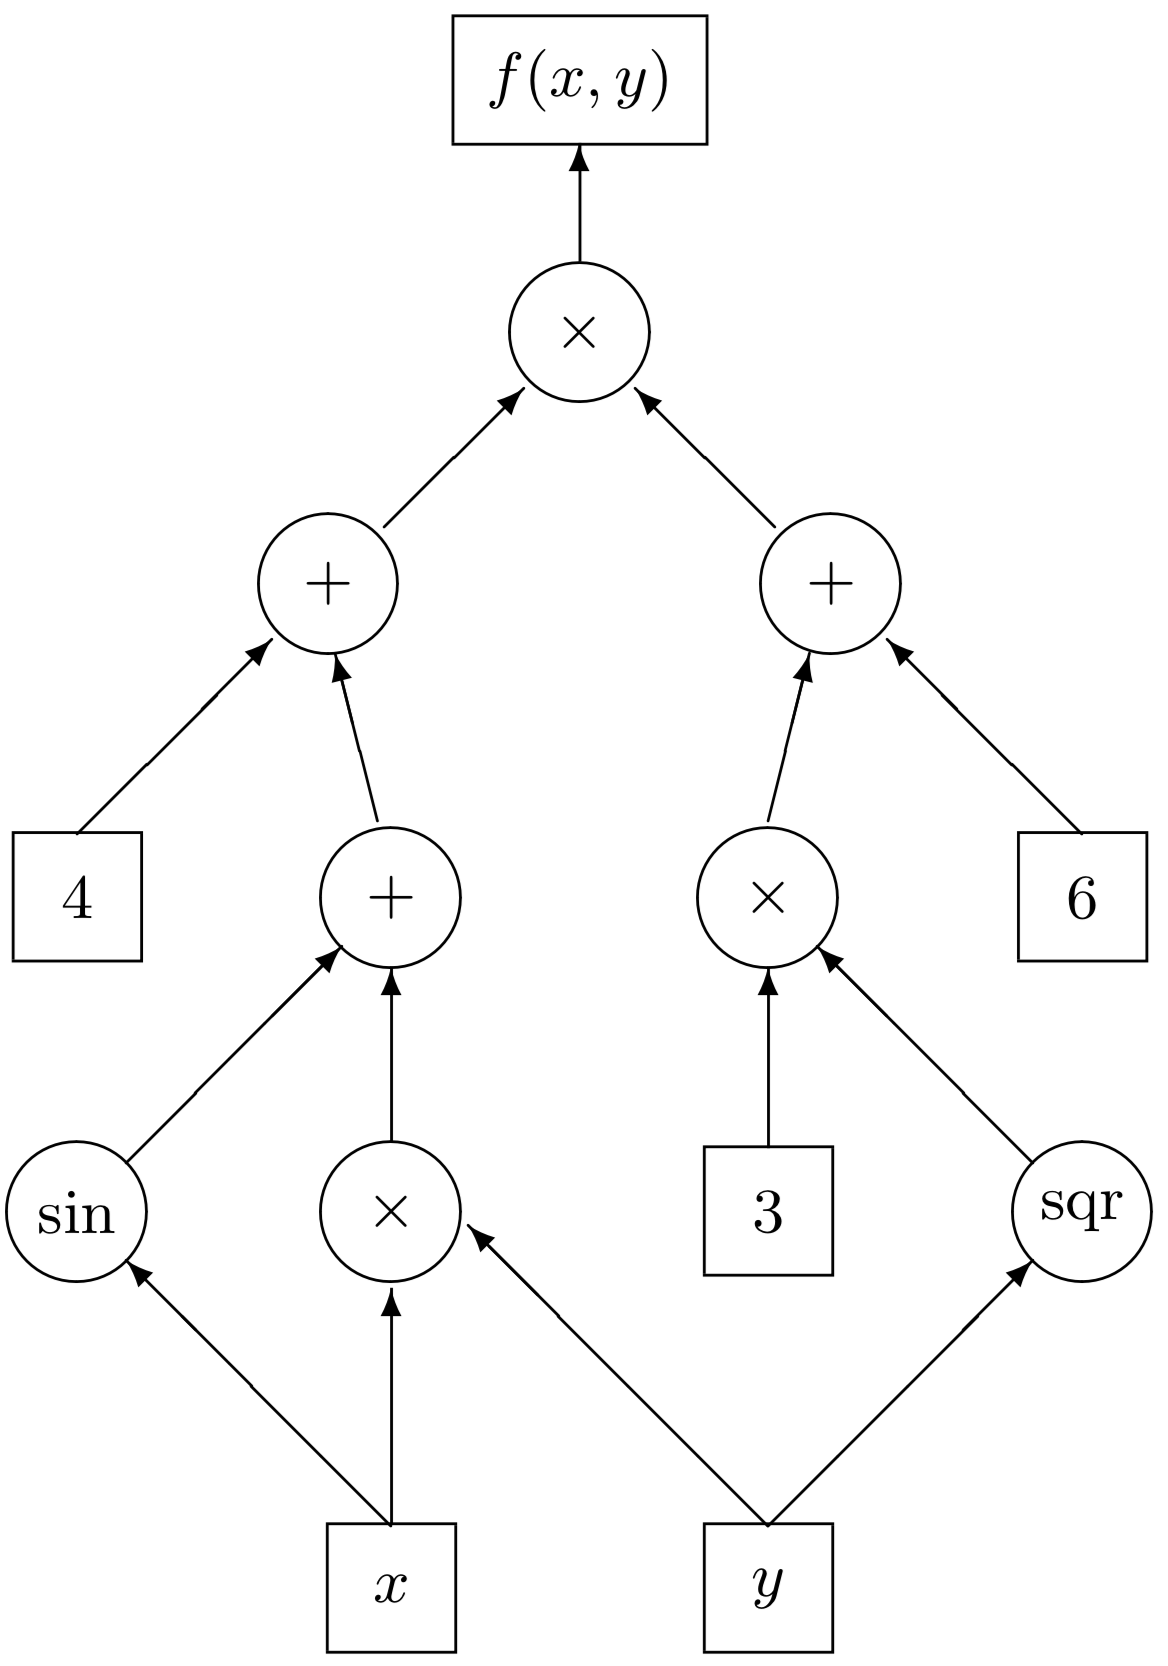
\includegraphics[scale=0.4]{Computational_graph}
\caption[Computational graph]{Computational graph\footnotemark}
\label{Computational_graph}
\end{figure} 

\footnotetext{Source: \citet{bucker2006automatic}}

In simple terms, a computation graph is a DAG in which nodes represent variables (tensors, matrix, scalars, etc.) and edge represent some mathematical operations (for example, summation, multiplication). The computation graph has some leaf variables. The root variables of the graph are computed according to operations defined by the graph. During the optimization step, we combine the chain rule and the graph to compute the derivative of the output w.r.t the learnable variable in the graph and update these variables.

There are two different modes of automatic differentiation, based on the application of the chain rule. The next section will start with forward mode automatic differentiation, which often is find a little more intuitive, described on the simple example.

\subsection{Forward mode}

Given a function $f$, one can construct a computational graph (a directed acyclic one) representing it, for instance let:

\[ f(x,y) = \cos(x) \sin(y) + \dfrac{x}{y} \]

Then each node of the graph represents a primitive function, while the edges represent the flow of information:

\begin{figure}[H]
\centering
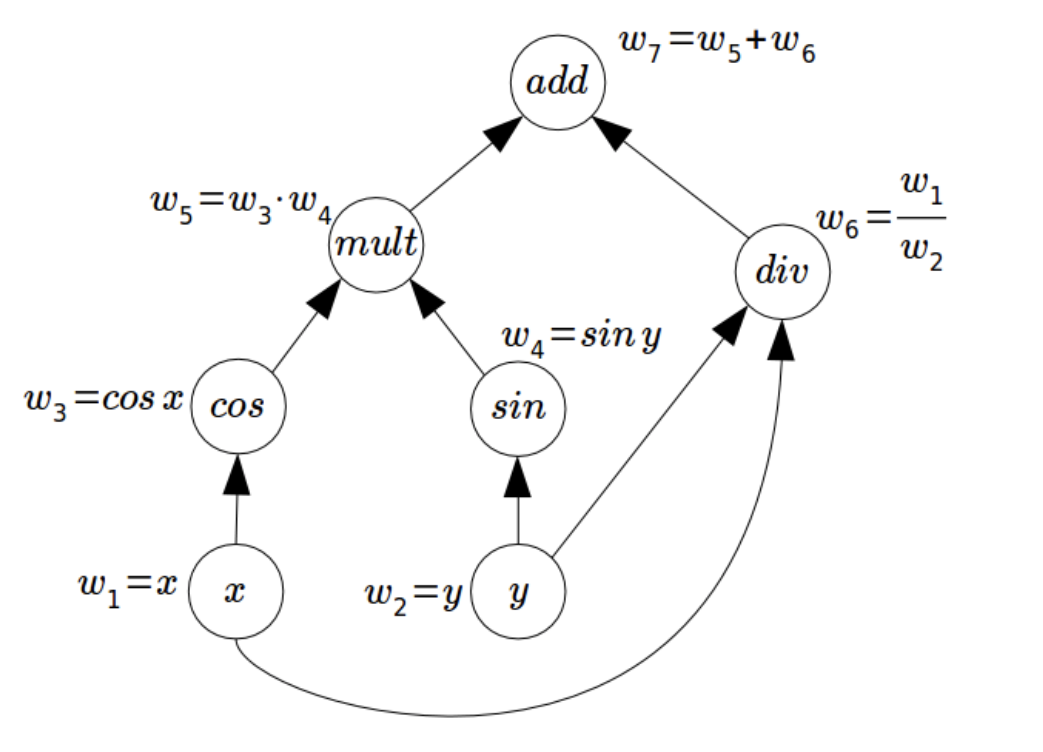
\includegraphics[width=0.8\textwidth,height=0.8\textheight,keepaspectratio]{Aut_diff}
\caption[Forward propagation]{Forward propagation\footnotemark}
\label{Forward_propagation}
\end{figure}

\footnotetext{Source: \url{http://www.columbia.edu/~ahd2125/post/2015/12/5/}}

Forward differentiation works by recursively defining derivatives of nodes in terms of their parents. Suppose one wants to calculate the partial $\dfrac{\partial f}{\partial x}$, denoted by $Df$. Then:

\begin{align*}
& Df = Dw_{7} = D(w_{5} + w_{6}) = Dw_{5} + Dw_{6} \\
& Dw_{6} = D\dfrac{w_{1}}{w_{2}} = \dfrac{w_{1}Dw_{2}- w_{2}Dw_{1}}{w_{2}^{2}}  \\
& Dw_{5} = Dw_{3}w_{4} = w_{3}Dw_{4} + w_{4}Dw_{3} \\
& Dw_{4} = D\sin(w_{2}) = \cos(w_{2}) Dw_{2} \\
& Dw_{3} = D\cos(w_{1}) = -\sin(w_{1}) Dw_{1} \\
& Dw_{2} = Dy \\
& Dw_{1} = Dx 
\end{align*}

The final value of $Df$ depends only on $x, y, Dw_{1}, Dw_{2}$. In this case, $ D = \dfrac{\partial f}{\partial x}$, so $Dx = 1$ and $Dy = 0$. Because information flows in the same direction as when one evaluates the expression (bottom-up), it is called the \textit{forward mode}. Predictably, the information flows top-down in  \textit{backward mode}, also called \textit{reverse mode}.

\subsection{Backward mode}

Reverse mode automatic differentiation lets calculate gradients much more efficiently than forward mode automatic differentiation. Suppose one wants to calculate the gradient:

\[ \triangledown f = \left<\frac{\partial f}{\partial x}, \frac{\partial f}{\partial y}\right> = \left<\frac{\partial w_{7}}{\partial w_{1}}, \frac{\partial w_{7}}{\partial w_{2}}\right> \]

Then:

\begin{align*}
& \frac{\partial w_{7}}{\partial w_{1}} = \frac{\partial w_{3}}{\partial w_{1}} \frac{\partial w_{7}}{\partial w_{3}} + \frac{\partial w_{6}}{\partial w_{1}} \frac{\partial w_{7}}{\partial w_{6}} = -\sin w_{1} \frac{\partial w_{7}}{\partial w_{3}} + \frac{1}{w_{2}} \frac{\partial w_{7}}{\partial w_{6}} \\
& \frac{\partial w_{7}}{\partial w_{2}} = \frac{\partial w_{4}}{\partial w_{2}} \frac{\partial w_{7}}{\partial w_{4}} + \frac{\partial w_{6}}{\partial w_{2}} \frac{\partial w_{7}}{\partial w_{6}} = \cos w_{2} \frac{\partial w_{7}}{\partial w_{4}} - \frac{w_{1}}{w_{2}^{2}} \frac{\partial w_{7}}{\partial w_{6}} \\
& \frac{\partial w_{7}}{\partial w_{3}} = \frac{\partial w_{5}}{\partial w_{3}} \frac{\partial w_{7}}{\partial w_{5}} = w_{4} \frac{\partial w_{7}}{\partial w_{5}} \\
& \frac{\partial w_{7}}{\partial w_{4}} = \frac{\partial w_{5}}{\partial w_{4}} \frac{\partial w_{7}}{\partial w_{5}} = w_{3} \frac{\partial w_{7}}{\partial w_{4}} \\
& \frac{\partial w_{7}}{\partial w_{5}} = 1 \\
& \frac{\partial w_{7}}{\partial w_{6}} = 1
\end{align*}

Instead of using the chain rule to find derivatives of parents in terms of derivatives of their children, one finds derivatives of children nodes in terms of their parents. Because information flows top-down, the reverse of normal evaluation, it is called the \textit{reverse mode} automatic differentiation.

Notice that  all operations in reverse mode differentiation are scalar operations, even though one calculates the (vector) gradient. Computing gradients via reverse mode can be thus significantly faster if $f$ contains a vast number of input variables.

\section{Tensor platform}

PyTorch is a relatively new deep learning library which support dynamic computation graphs and tensors which can tap into the resources of a GPU to significantly speed up matrix operations. The dynamic graph paradigm allows to make changes to the model architecture during runtime, as a graph is created only when a piece of code is run. This means a graph may be redefined during the lifetime for a program. This, however, is not possible with static graphs, used by another popular deep learning libraryTensorFlow, where graphs are created before running the program, and merely executed later. 

Finally, PyTorch has in-built several optimization algorithms, such as Stochastic Gradient Descent or ADAM, which solves the likelihood maximization problem relatively costlessly.

\chapter{Results}

Here go the results.


\chapter{Concluding remarks} \label{Concluding remarks}

Here goes the conclusion.

Potential extensions: GPU acceleration, higher approximations

\newpage

\nocite{*}
\addcontentsline{toc}{chapter}{Bibliography}
\bibliography{Dissertation}

\newpage

\chapter*{Appendix A} \label{Appendix A}
\addcontentsline{toc}{chapter}{Appendix A}

\section*{Consumption and savings behavior}

The maximization of the objective function of the household subject to the budget constraint with respect to consumption and holdings of bonds, may be performed through the Lagrangian-based technique:

\begin{equation}
\begin{split}
L = \mathbb{E}_{0} \sum\limits_{t=0}^{\infty} \beta^{t} \varepsilon_{t}^{B} \left[ \frac{1}{1-\sigma_{c}} \left( C_{t}^{\tau} - H_{t}^{\tau} \right)^{1-\sigma_{c}} - \frac{\varepsilon_{t}^{L}}{1+\sigma_{l}} \left( l_{t}^{\tau} \right)^{1+\sigma_{l}} \right] + \\
- \beta^{t} \lambda_{t} \left[ C_{t}^{\tau} + I_{t}^{\tau} + b_{t} \frac{B_{t}^{\tau}}{P_{t}} - Y_{t}^{\tau} - \frac{B_{t-1}^{\tau}}{P_{t}} \right]
\end{split}
\end{equation}

The derivatives with respect to $C_{t}^{\tau}$ and $B_{t}^{\tau}$ are respectively:

\begin{align}
\frac{\partial L}{\partial C_{t}^{\tau}} &= \mathbb{E}_{t} \left[ \beta^{t} \left( \varepsilon_{t}^{B} (
C_{t}^{\tau} - H_{t} )^{-\sigma_{c}} - \lambda_{t} \right) \right]  = 0  \nonumber \\ 
& \iff \lambda_{t} =  \varepsilon_{t}^{B} (C_{t}^{\tau} - H_{t} )^{-\sigma_{c}} = \frac{\partial U_{t}^{\tau}}{\partial C_{t}^{\tau}} := U_{t}^{c} \label{FOC_C} \\
\frac{\partial L}{\partial B_{t}^{\tau}} &= -\mathbb{E}_{t} \left[ \beta^{t} \lambda_{t} \frac{b_{t}}{P_{t}} \right] - \mathbb{E}_{t} \left[ \beta^{t+1} \lambda_{t+1} \frac{-1}{P_{t+1}} \right] = 0 \nonumber \\
& \iff \mathbb{E}_{t} \left[ \beta \frac{\lambda_{t+1}}{\lambda_{t}} \frac{1}{b_{t}} \frac{P_{t}}{P_{t+1}} \right] = 1 \label{FOC_B} 
\end{align}

Exploiting the fact that households are homogeneous in their consumption-saving decisions,  meaning that the marginal utility of consumption is identical for all $\tau$, yields the following Euler equation:

\begin{align}
\mathbb{E}_{t} \left[ \beta \frac{\lambda_{t+1}}{\lambda_{t}} \frac{1}{b_{t}}\frac{P_{t}}{P_{t+1}} \right] &= \mathbb{E}_{t} \left[ \beta \frac{U^{c}_{t+1}}{U^{c}_{t}} (1 + i_{t}) \frac{P_{t}}{P_{t+1}} \right] = \nonumber \\
&= \mathbb{E}_{t} \left[ \beta \frac{\varepsilon_{t+1}^{B} (C_{t+1}^{\tau} - H_{t+1} )^{-\sigma_{c}}}{\varepsilon_{t}^{B} (C_{t}^{\tau} - H_{t} )^{-\sigma_{c}}} R_{t} \frac{P_{t}}{P_{t+1}} \right] = \nonumber \\
&= \mathbb{E}_{t} \left[ \beta \frac{\varepsilon_{t+1}^{B} (C_{t+1}^{\tau} - h \cdot C_{t} )^{-\sigma_{c}}}{\varepsilon_{t}^{B} (C_{t}^{\tau} - h \cdot C_{t-1} )^{-\sigma_{c}}} R_{t} \frac{P_{t}}{P_{t+1}} \right] = 1
\end{align}

Alternatively one can rearrange the aforementioned equation as:
\begin{align}
\mathbb{E}_{t} \left[ \beta \frac{\lambda_{t+1}}{\lambda_{t}} \frac{1}{b_{t}}\frac{P_{t}}{P_{t+1}} \right] &= \mathbb{E}_{t} \left[ \beta \frac{U^{c}_{t+1}}{U^{c}_{t}} (1 + i_{t}) \frac{P_{t}}{P_{t+1}} \right] = 1 \nonumber \\
& \iff \beta (1 + i_{t}) \mathbb{E}_{t} \left[ \frac{U_{t+1}^{c}}{P_{t+1}} \right] = \frac{U_{t}^{c}}{P_{t}}
\end{align}

\section*{Labor supply decisions}

The problem of the firm is as following:

\begin{align}
\min_{l_{t}^{\tau}} \int\limits_{0}^{1} W_{t}^{\tau} l_{t}^{\tau} d\tau \quad \text{s.t.} \quad L_{t} = \left[ \int\limits_{0}^{1} \left( l_{t}^{\tau} \right)^{\frac{1}{1+\lambda_{w,t}}} d\tau \right]^{1+\lambda_{w,t}}
\end{align}

Define $W_{t}$ as the Lagrange multiplier, then the cost minimization becomes:

\begin{align}
L = \int\limits_{0}^{1} W_{t}^{\tau} l_{t}^{\tau} d\tau + W_{t} \left( L_{t} - \left[ \int\limits_{0}^{1} \left( l_{t}^{\tau} \right)^{\frac{1}{1+\lambda_{w,t}}} d\tau \right]^{1+\lambda_{w,t}} \right)
\end{align}

Taking the first order conditions:

\begin{align} \label{Optimal demand function for labor}
\frac{\partial L}{\partial l_{t}^{\tau}} &= W_{t}^{\tau} - W_{t} \left( \left( 1+\lambda_{w ,t} \right) \left[  \int\limits_{0}^{1} \left( l_{t}^{\tau} \right)^{\frac{1}{1+\lambda_{w ,t}}} d\tau \right]^{\lambda_{w ,t}} \frac{1}{1+\lambda_{w ,t}}  \left( l_{t}^{\tau} \right)^{\frac{-\lambda_{w ,t}}{1+\lambda_{w ,t}}} \right) = 0 \nonumber \\
& \iff W_{t}^{\tau} = W_{t} L_{t}^{\frac{\lambda_{w ,t}}{1+\lambda_{w,t}}} \left( l_{t}^{\tau} \right)^{\frac{-\lambda_{w,t}}{1+\lambda_{w ,t}}} \nonumber \\
& \iff l_{t}^{\tau}= L_{t} \left( \frac{W_{t}^{\tau}}{W_{t}}\right)^{\frac{-(1+\lambda_{w,t})}{\lambda_{w ,t}}}
\end{align} 

The derived optimal demand function of labor can be then substituted in the aggregate labor demand equation yielding:

\begin{align}
L_{t} &= \left[ \int\limits_{0}^{1} \left( \frac{W_{t}^{\tau}}{W_{t}}\right)^{\frac{-1}{\lambda_{w ,t}}} L_{t}^{\frac{1}{1+\lambda_{w ,t}}} d\tau \right]^{1+\lambda_{w,t}} \nonumber \\
& \iff W_{t} = \left[ \int\limits_{0}^{1} \left( W_{t}^{\tau} \right)^{\frac{-1}{\lambda_{w ,t}}}  d\tau \right]^{-\lambda_{w,t}}
\end{align}

The Lagrange multiplier $W_{t}$, generally considered as the representation of the marginal value of relaxing the constrain, can be interpreted as well as the price of a working hour and thus a wage index.

\section*{Wage setting equation}

Households that can re-set their wages maximize their objective function subject to their budget constraint and the demand of labor, taking into consideration the fact that wages remain fixed until period $i$ with a probability $\left( \varsigma_{w} \right)^{i}$. The Lagrangian function in t becomes:

\begin{align}
L = \mathbb{E}_{t} \sum\limits_{i=0}^{\infty} &\beta^{i} \varsigma_{w}^{i} \left\{\underbrace{U \left(C_{t+i}^{\tau}, l_{t+i}^{\tau} \right)}_\text{Utility function} - \lambda_{t+i} \left( \underbrace{\ldots + \frac{W_{t+i}^{\tau}}{P_{t+i}} l_{t+i}^{\tau} + \ldots }_\text{Budget constraint} \right) + \nonumber \right. \\ 
& \left. - \mu_{t+i} \left( \underbrace{l_{t+i}^{\tau} - L_{t+i}^{\tau} \left(\frac{W_{t+i}^{\tau}}{W_{t+i}} \right)^{\frac{-\left(1-\lambda_{w, t+i}\right)}{\lambda_{w, t+i}}}}_\text{Labor demand} \right) \right\}
\end{align}

Substituting the demand of labour (\ref{Optimal demand function for labor}) in the objective function and in the budget constraint and considering the formulas for not reoptimized wages in period $t+i$, one obtains:

\begin{align}
L = \mathbb{E}_{t} \sum\limits_{i=0}^{\infty} &\beta^{i} \varsigma_{w}^{i}  \left\{ \underbrace{U \left(C_{t+i}^{\tau}, L_{t+i} \left( \frac{\left( \frac{P_{t+i-1}}{P_{t-1}} \right)^{\gamma_{w}} \widetilde{W}_{t}}{W_{t+i}}\right)^{\frac{-(1+\lambda_{w,t+i})}{\lambda_{w,t+i}}} \right)}_\text{Utility function} + \right. \nonumber \\
& \left. - \lambda_{t+i} \left( \underbrace{\ldots + \left( \frac{P_{t+i-1}}{P_{t-1}} \right)^{\gamma_{w}} \frac{\widetilde{W}_{t}}{P_{t+i}} L_{t+i} \left( \frac{\left( \frac{P_{t+i-1}}{P_{t-1}} \right)^{\gamma_{w}} \widetilde{W}_{t}}{W_{t+i}}\right)^{\frac{-(1+\lambda_{w,t+i})}{\lambda_{w,t+i}}}
 + \ldots }_\text{Budget constraint} \right) \right\}
\end{align}

Taking the first order conditions:

\begin{align}
\frac{\partial L}{\partial \widetilde{W}_{t}}  =  \mathbb{E}_{t} \sum\limits_{i=0}^{\infty} &\beta^{i} \varsigma_{w}^{i}  \left\{ U_{t+i}^{L} {\frac{-(1+\lambda_{w,t+i})}{\lambda_{w,t+i}}} L_{t+i} \left( \frac{\left( \frac{P_{t+i-1}}{P_{t-1}} \right)^{\gamma_{w}} \widetilde{W}_{t}}{W_{t+i}}\right)^{\frac{-(1+\lambda_{w,t+i})}{\lambda_{w,t+i}}-1} \left( \frac{\left( \frac{P_{t+i-1}}{P_{t-1}} \right)^{\gamma_{w}}}{W_{t+i}}\right)  \right. + \nonumber \\ 
-  &\lambda_{t+i} \left[ \left( \frac{P_{t+i-1}}{P_{t-1}} \right)^{\gamma_{w}} \frac{1}{P_{t+i}} L_{t+i} \left( \frac{\left( \frac{P_{t+i-1}}{P_{t-1}} \right)^{\gamma_{w}} \widetilde{W}_{t}}{W_{t+i}}\right)^{\frac{-(1+\lambda_{w,t+i})}{\lambda_{w,t+i}}} \right. + \nonumber \\ 
-  &\left. \left. \left( \frac{P_{t+i-1}}{P_{t-1}} \right)^{\gamma_{w}} \frac{\widetilde{W_{t}}}{P_{t+i}} L_{t+i} {\frac{1+\lambda_{w,t+i}}{\lambda_{w,t+i}}} \left( \frac{\left( \frac{P_{t+i-1}}{P_{t-1}} \right)^{\gamma_{w}} \widetilde{W}_{t}}{W_{t+i}}\right)^{\frac{-(1+\lambda_{w,t+i})}{\lambda_{w,t+i}}-1} \left( \frac{\left( \frac{P_{t+i-1}}{P_{t-1}} \right)^{\gamma_{w}}}{W_{t+i}}\right) \right] \right\} = 0
\end{align}

Therefore:

\begin{align}
\frac{\partial L}{\partial \widetilde{W}_{t}} = &\mathbb{E}_{t} \sum\limits_{i=0}^{\infty} \beta^{i} \varsigma_{w}^{i}  \left\{ U_{t+i}^{L} {\frac{-(1+\lambda_{w,t+i})}{\lambda_{w,t+i}}} \frac{l_{t+1}^{\tau}}{\widetilde{W}_{t}}  \right. + \nonumber \\ 
- &\lambda_{t+i} \left. \left[ \left( \frac{P_{t+i-1}}{P_{t-1}} \right)^{\gamma_{w}} \frac{1}{P_{t+i}} l_{t+i}^{\tau} - {\frac{1+\lambda_{w,t+i}}{\lambda_{w,t+i}}} \left( \frac{P_{t+i-1}}{P_{t-1}} \right)^{\gamma_{w}} \frac{1}{P_{t+i}} l_{t+i}^{\tau} \right] \right\} = \nonumber \\ 
= &\mathbb{E}_{t} \sum\limits_{i=0}^{\infty} \beta^{i} \varsigma_{w}^{i}  \left\{ U_{t+i}^{L} {\frac{-(1+\lambda_{w,t+i})}{\lambda_{w,t+i}}} \frac{l_{t+1}^{\tau}}{\widetilde{W}_{t}}  \right. + \nonumber \\ 
- &\lambda_{t+i} \left. \left[ {\frac{-1}{\lambda_{w,t+i}}} \left( \frac{P_{t+i-1}}{P_{t-1}} \right)^{\gamma_{w}} \frac{1}{P_{t+i}} l_{t+i}^{\tau} \right] \right\} = 0
\end{align}

Multiplying by the factor $\frac{-\lambda_{w,t+i}}{1+\lambda_{w,t+i}}$ and considering that $\lambda_{t} = U_{t}^{c}$ one obtains:

\begin{align}
\frac{\widetilde{W}_{t}}{P_{t}} &\mathbb{E}_{t} \left\{ \sum\limits_{i=0}^{\infty} \beta^{i} \varsigma_{w}^{i} \left( \frac{P_{t+i-1}}{P_{t-1}} \right)^{\gamma_{w}}  \frac{P_{t}}{P_{t+i}} \left( \frac{l_{t+1}^{\tau} U_{t+i}^{C}}{1 + \lambda_{w, t+i}} \right) \right\} = \nonumber \\
&= \mathbb{E}_{t} 
\left\{ \sum\limits_{i=0}^{\infty} \beta^{i} \varsigma_{w}^{i} l_{t+1}^{\tau} U_{t+i}^{l} \right\}
\end{align}

Assuming perfect flexibility of wages $(\varsigma_{w} = 0)$, the above-mentioned equation becomes:

\begin{align}
\frac{\widetilde{W}_{t}}{P_{t}} = \left(1 + \lambda_{w, t} \right)\frac{U_{t}^{L}}{U_{t}^{C}}
\end{align}

\section*{Capital accumulation and investment decision}

Define the Lagrange multiplier $\lambda_{t} Q_{t}$ for the maximization problem with respect to $K_{t}, I_{t}, z_{t}$:

\begin{align}
L = \mathbb{E}_{0} \sum\limits_{t=0}^{\infty} &\beta^{t} \left[\underbrace{U \left(C_{t}^{\tau}, l_{t}^{\tau} \right)}_\text{Objective function} - \lambda_{t} \left( \underbrace{I_{t} + \left(\Psi(z_{t}) - r_{t}^{k}z_{t}\right)K_{t-1} + \ldots}_\text{Budget constraint} \right) + \nonumber \right.  \\ 
& \left. - \lambda_{t} Q_{t} \left( \underbrace{K_{t} - K_{t-1} (1 - \tau) - I_{t}  + I_{t} \cdot S \left(\frac{\varepsilon_{t}^{I}I_{t}}{I_{t-1}} \right)}_\text{Capital accumulation} \right) \right]
\end{align}

The first-order conditions:

\begin{align}
\frac{\partial L}{\partial z_{t}} &= \mathbb{E}_{t} \left[ -\beta^{t} \lambda_{t} \left( \Psi'(z_{t}) - r_{t}^{k} \right) K_{t-1} \right] = 0 \nonumber \\
& \iff r_{t}^{k} = \Psi'(z_{t})
\end{align}

The capital utilization rate is set so that the revenue $r_{t}^{k}$ of the marginal utilization equals the marginal costs $\Psi'(z_{t})$.

\begin{align}
\frac{\partial L}{\partial K_{t}} &= \mathbb{E}_{t} \left[ \beta^{t+1} \lambda_{t+1} \left( z_{t+1}r_{t+1}^{k} - \Psi(z_{t+1}) \right) - \beta^{t} \lambda_{t}Q_{t} + \beta^{t+1} \lambda_{t+1}Q_{t+1}(1-\tau) \right] = 0 \nonumber \\
& \iff Q_{t} = \mathbb{E}_{t} \left[ \beta \frac{\lambda_{t+1}}{\lambda_{t}} \left( Q_{t+1}(1-\tau) + z_{t+1}r_{t+1}^{k} - \Psi(z_{t+1}) \right) \right]
\end{align}

The real value of the stock of capital today $\lambda_{t} Q_{t}$ is equal to the expected value of sum of not depreciated stock of capital of the next period $\lambda_{t+1}Q_{t+1}(1-\tau)$ and the expected revenue of the future utilization $ z_{t+1}r_{t+1}^{k}$ minus the related costs $\Psi(z_{t+1})$.

\begin{align}
\frac{\partial L}{\partial I_{t}} &= \mathbb{E}_{t} \left[ -\beta^{t} \lambda_{t} - \beta^{t} \lambda_{t} Q_{t} \left(-1 + S\left(\frac{\varepsilon_{t}^{I}I_{t}}{I_{t-1}} \right) + I_{t} \cdot S' \left(\frac{\varepsilon_{t}^{I}I_{t}}{I_{t-1}} \right) \cdot \frac{\varepsilon_{t}^{I}}{I_{t-1}} \right) \right] + \nonumber \\
\qquad &- \mathbb{E}_{t} \left[ \beta^{t+1} \lambda_{t+1} Q_{t+1} \left(I_{t+1} \cdot S' \left(\frac{\varepsilon_{t+1}^{I}I_{t+1}}{I_{t}} \right) \cdot \frac{-\varepsilon_{t+1}^{I}I_{t+1}}{I_{t}^{2}} \right) \right] = 0
\end{align}

The costs of the marginal investment (included the adjustment costs) must be equal to the expected marginal revenue of investment.

\section*{Firms - Final product sector}

The Lagrangian for the minimization problem:

\begin{align}
\int\limits_{0}^{1} p_{t}^{j} y_{t}^{j}dj + P_{t} \left( Y_{t} - \left[ \int\limits_{0}^{1} \left(y_{t}^{j} \right)^\frac{1}{1+\lambda_{p,t}} dj \right]^{1+\lambda_{p,t}} \right)
\end{align}

First order conditions:

\begin{align}
\frac{\partial L}{\partial y_{t}^{j}} &= p_{t}^{j} - P_{t} \left( \left( 1+\lambda_{p,t} \right) \left[ \int\limits_{0}^{1} \left(y_{t}^{j} \right)^\frac{1}{1+\lambda_{p,t}} dj \right]^{\lambda_{p,t}} \frac{1}{1+\lambda_{p,t}} \left( y_{t}^{j} \right)^{ \frac{-\lambda_{p,t}}{1+\lambda_{p,t}}} \right) = 0 \nonumber \\
&  \iff p_{t}^{j} = P_{t}  Y_{t}^{ \frac{\lambda_{p,t}}{1+\lambda_{p,t}}} \left( y_{t}^{j} \right)^{ \frac{-\lambda_{p,t}}{1+\lambda_{p,t}}} \nonumber \\
& \iff y_{t}^{j} = Y_{t} \left( \frac{p_{t}^{j}}{P_{t}} \right)^{ \frac{-(1+\lambda_{p,t})}{\lambda_{p,t}}} 
\end{align}

Substituting into the technology constraint:

\begin{align}
Y_{t} &=  \left[ \int\limits_{0}^{1} \left( \frac{ p_{t}^{j}}{P_{t}} \right)^{\frac{-1}{\lambda_{p,t}}} Y_{t}^\frac{1}{1+\lambda_{p,t}} dj \right]^{1+\lambda_{p,t}} \nonumber \\
& \iff P_{t} = \left[ \int\limits_{0}^{1} \left( p_{t}^{j} \right)^{\frac{-1}{\lambda_{p,t}}} dj \right]^{-\lambda_{p,t}}
\end{align}


\section*{Firms - Intermediate product sector}

In order to find the optimal production quantity, it is convenient to show that marginal costs are constant. One proceeds first by finding a functional relationship between $\widetilde{K}_{j,t}$ and $L_{j,t}$ derived by the minimization problem of $W_{t}L_{j,t} + r_{t}^{k} \widetilde{K}_{j,t}$ with respect to $L_{j,t}$ and $\widetilde{K}_{j,t}$ subject to $y_{t}^{j} = \varepsilon_{t}^{a} \widetilde{K}_{j,t}^{\alpha} L_{j,t}^{1-\alpha} - \Phi$.

\begin{align}
\frac{W_{t}}{r_{t}^{k}} &= \frac{(1-\alpha)\varepsilon_{t}^{a} \widetilde{K}_{j,t}^{\alpha} L_{j,t}^{-\alpha} }{\alpha \varepsilon_{t}^{a} \widetilde{K}_{j,t}^{\alpha-1} L_{j,t}^{1-\alpha} } \nonumber \\
& \iff \frac{W_{t}L_{t,j}}{r_{t}^{k}  \widetilde{K}_{j,t}} = \frac{1-\alpha}{\alpha}
\end{align}

The utilization rate between capital and labour is identical for all firms and constant. This is the same of the economy as a whole. The marginal costs of product $j$ are derived by substituting the above-mentioned relation in the production function:

\begin{align}
\widetilde{K}_{j,t} &= \left(y_{t}^{j} + \Phi \right) \frac{1}{\varepsilon_{t}^{a}} \left(\frac{\alpha}{1-\alpha} \frac{W_{t}}{r_{t}^{k}} \right)^{1-\alpha} \\
L_{j,t} &= \left(y_{t}^{j} + \Phi \right) \frac{1}{\varepsilon_{t}^{a}} \left(\frac{\alpha}{1-\alpha} \frac{W_{t}}{r_{t}^{k}} \right)^{-\alpha}
\end{align}

Therefore the total cost equals:

\begin{align}
TC_{t} = W_{t}L_{j,t}  + r_{t}^{k} \widetilde{K}_{j,t} =  \left(y_{t}^{j} + \Phi \right) \frac{1}{\varepsilon_{t}^{a}} W_{t}^{1-\alpha} \left(r_{t}^{k} \right)^{\alpha} \left( \alpha^{-\alpha} (1-\alpha)^{-(1-\alpha)}\right)
\end{align}

Hence the marginal cost takes the form:

\begin{align}
MC_{t} = \frac{\partial TC_{t}}{\partial y_{t}^{j}} = \frac{1}{\varepsilon_{t}^{a}} W_{t}^{1-\alpha} \left(r_{t}^{k} \right)^{\alpha} \left( \alpha^{-\alpha} (1-\alpha)^{-(1-\alpha)}\right)
\end{align}

In order to derive the optimal mark-up formula for the reoptimize price, the Lagrangian can be formed:

\begin{align}
L = \mathbb{E}_{t}  \sum\limits_{i=0}^{\infty} \beta^{i} \varsigma_{p}^{i} \rho_{t+i} \left\{ \left[
\left(\frac{P_{t+i-1}}{P_{t-1}} \right)^{\gamma_{p}}\widetilde{p}_{t} - MC_{t+i}
\right] Y_{t+i} \left[ \frac{\left(\frac{P_{t+i-1}}{P_{t-1}} \right)^{\gamma_{p}}\widetilde{p}_{t}}{P_{t+i}} \right]^{\frac{-(1+\lambda_{p,t+i})}{\lambda_{p,t+i}}} - \Phi MC_{t+i} \right\}
\end{align}

First order condition:

\begin{align}
\frac{\partial L}{\partial \widetilde{p}_{t}} &= \mathbb{E}_{t}  \sum\limits_{i=0}^{\infty} \beta^{i} \varsigma_{p}^{i} \rho_{t+i} \left\{ \left[
\left(\frac{P_{t+i-1}}{P_{t-1}} \right)^{\gamma_{p}} \right] Y_{t+i} \left[ \frac{\left(\frac{P_{t+i-1}}{P_{t-1}} \right)^{\gamma_{p}}\widetilde{p}_{t}}{P_{t+i}} \right]^{\frac{-(1+\lambda_{p,t+i})}{\lambda_{p,t+i}}} \right. + \nonumber \\
& \left. + \left[\left(\frac{P_{t+i-1}}{P_{t-1}} \right)^{\gamma_{p}}\widetilde{p}_{t} -MC_{t+i} \right] Y_{t+i} \frac{-(1+\lambda_{p,t+i})}{\lambda_{p,t+i}} \left[ \frac{\left(\frac{P_{t+i-1}}{P_{t-1}} \right)^{\gamma_{p}}\widetilde{p}_{t}}{P_{t+i}} \right]^{\frac{-(1+\lambda_{p,t+i})}{\lambda_{p,t+i}}-1} \frac{\left(\frac{P_{t+i-1}}{P_{t-1}} \right)^{\gamma_{p}}}{P_{t+i}} \right\} = \nonumber \\
& = \mathbb{E}_{t}  \sum\limits_{i=0}^{\infty} \beta^{i} \varsigma_{p}^{i} \rho_{t+i} \left\{ \left[ \left(\frac{P_{t+i-1}}{P_{t-1}} \right)^{\gamma_{p}} \right] y^{j}_{t+i} + \left[\left(\frac{P_{t+i-1}}{P_{t-1}} \right)^{\gamma_{p}}\widetilde{p}_{t} -MC_{t+i} \right] \frac{-(1+\lambda_{p,t+i})}{\lambda_{p,t+i}} \frac{y_{t+i}^{j}}{\widetilde{p}_{t}} \right\} = 0
\end{align}

Multiplying through the factor $\widetilde{p}_{t} \lambda_{p,t+i}$ and considering equation \ref{Euler for firm}, the following mark-up formula for the reoptimized price obtains:

\begin{align}
&\mathbb{E}_{t}  \sum\limits_{i=0}^{\infty} \beta^{i} \varsigma_{p}^{i} \frac{\lambda_{t+i}}{\lambda_{t}} y_{t+i}^{j} \left\{ \frac{\widetilde{p}_{t}}{P_{t}} \left[ \frac{ \left(\frac{P_{t+i-1}}{P_{t-1}} \right)^{\gamma_{p}}}{\frac{P_{t+i}}{P_{t}}} \right] - (1+\lambda_{p,t+i})\frac{MC_{t+i}}{P_{t+i}} \right\} = 0
\end{align}

\section*{Log-linearised DSGE model - Consumption}

Recall that:

\begin{align}
\lambda_{t} = \varepsilon_{t}^{B} \left( C_{t}^{\tau} - H_{t} \right)^{-\sigma_{c}}
\end{align}

Then from the household maximization problem it holds that:

\begin{align}
& \mathbb{E}_{t} \left[\beta \lambda_{t+1} \frac{R_{t}}{P_{t+1}} \right] = \frac{\lambda_{t}}{P_{t}} 
\end{align}

Then the left-hand side:

\begin{align}
& \mathbb{E}_{t} \left[\beta \lambda_{t+1} \frac{R_{t}}{P_{t+1}} \right]  \nonumber \\
& = \mathbb{E}_{t} \left[\beta \varepsilon_{t+1}^{B} \left( C_{t+1}^{\tau} - H_{t+1} \right)^{-\sigma_{c}} \frac{R_{t}}{P_{t+1}} \right] = \nonumber \\
& = \mathbb{E}_{t} \left[\beta \varepsilon_{t+1}^{B} \left( C_{t+1}^{\tau} - h C_{t} \right)^{-\sigma_{c}} \frac{R_{t}}{P_{t+1}} \right] \simeq \nonumber \\
& \simeq \mathbb{E}_{t} \left[\beta \varepsilon^{B} \left( C - hC \right)^{-\sigma_{c}} \frac{R}{P} +  \beta \varepsilon^{B} \left( C - hC \right)^{-\sigma_{c}} \frac{R}{P} \hat{\varepsilon}_{t+1}^{B} - \sigma_{c}\beta \varepsilon^{B} \left( C - hC \right)^{-\sigma_{c}-1} \left(C \hat{C}_{t+1} - h C \hat{C}_{t} \right) \frac{R}{P} + \right. \nonumber \\
& \left. \qquad + \beta \varepsilon^{B} \left( C - hC \right)^{-\sigma_{c}} \frac{R}{P} \hat{R}_{t} - \beta \varepsilon^{B} \left( C - hC \right)^{-\sigma_{c}} \frac{R}{P} \hat{P}_{t+1} \right] = \nonumber \\
& = \mathbb{E}_{t} \left[\beta \varepsilon^{B} \left( C - hC \right)^{-\sigma_{c}} \frac{R}{P} \cdot \left( 1 +  \hat{\varepsilon}_{t+1}^{B} - \sigma_{c} \left(C - hC \right)^{-1} \left(C \hat{C}_{t+1} - hC \hat{C}_{t} \right) + \hat{R}_{t} - \hat{P}_{t+1} \right) \right]
\end{align}

While the right-hand side:

\begin{align}
\frac{\lambda_{t}}{P_{t}} &= \varepsilon_{t}^{B} \left( C_{t}^{\tau} - H_{t} \right)^{-\sigma_{c}}  P_{t}^{-1} =  \varepsilon_{t}^{B} \left( C_{t}^{\tau} - h C_{t-1} \right)^{-\sigma_{c}}  P_{t}^{-1} \simeq \nonumber \\
& \simeq \varepsilon^{B} \left( C - h C  \right)^{-\sigma_{c}}  P^{-1} +  \varepsilon^{B} \left( C - h C  \right)^{-\sigma_{c}}  P^{-1} \hat{\varepsilon}_{t}^{B} + \nonumber \\
& \qquad - \sigma_{C} \varepsilon^{B} \left( C - h C  \right)^{-\sigma_{c}-1}  P^{-1} \left(C \hat{C}_{t} - h C \hat{C}_{t-1} \right) + \nonumber \\
& \qquad - \varepsilon^{B} \left( C - h C  \right)^{-\sigma_{c}}  P^{-1} \hat{P}_{t} = \nonumber \\
& = \varepsilon^{B} \left( C - h C  \right)^{-\sigma_{c}}  P^{-1} \left( 1 + \hat{\varepsilon}_{t}^{B} - \sigma_{C} \left( C - h C  \right)^{-1} \left(C \hat{C}_{t} - h C \hat{C}_{t-1} \right) -\hat{P}_{t}
\right)
\end{align}

Finally considering that in the steady-state:

\begin{align}
\beta R \left[ \varepsilon^{B} \left( C - h C  \right)^{-\sigma_{c}} \right] &= \varepsilon^{B} \left( C - h C  \right)^{-\sigma_{c}} \frac{P}{P} \nonumber \\
\iff & \beta = \frac{1}{R}
\end{align}

Putting both sides together yields:

\begin{align}
\hat{R}_{t} + \mathbb{E}_{t} \hat{\varepsilon}^{B}_{t+1} - \frac{\sigma_{c}}{1-h} \left( \mathbb{E}_{t}\hat{C}_{t+1} - h \hat{C}_{t} \right) = \hat{\varepsilon}^{B}_{t} - \frac{\sigma_{c}}{1-h} \left( \hat{C}_{t} - h \hat{C}_{t-1} \right) + \mathbb{E}_{t} \hat{\Pi}_{t+1}
\end{align}

from which one obtains the explicit expression for $\hat{C}_{t}$.

\section*{Log-linearised DSGE model - Investment}

Recall the optimal condition for investment:

\begin{align}
\frac{\partial L}{\partial I_{t}} &= \mathbb{E}_{t} \left[ -\beta^{t} \lambda_{t} - \beta^{t} \lambda_{t} Q_{t} \left(-1 + S\left(\frac{\varepsilon_{t}^{I}I_{t}}{I_{t-1}} \right) + I_{t} \cdot S' \left(\frac{\varepsilon_{t}^{I}I_{t}}{I_{t-1}} \right) \cdot \frac{\varepsilon_{t}^{I}}{I_{t-1}} \right) \right] + \nonumber \\
\qquad &- \mathbb{E}_{t} \left[ \beta^{t+1} \lambda_{t+1} Q_{t+1} \left(I_{t+1} \cdot S' \left(\frac{\varepsilon_{t+1}^{I}I_{t+1}}{I_{t}} \right) \cdot \frac{-\varepsilon_{t+1}^{I}I_{t+1}}{I_{t}^{2}} \right) \right] = 0 \nonumber \\
& \iff Q_{t}S' \left(\frac{\varepsilon_{t}^{I}I_{t}}{I_{t-1}} \right) \left( \frac{\varepsilon_{t}^{I}I_{t}}{I_{t-1}} \right) - \beta \mathbb{E}_{t} \left[ Q_{t+1} \frac{\lambda_{t+1}}{\lambda_{t}} S' \left(\frac{\varepsilon_{t+1}^{I}I_{t+1}}{I_{t}} \right) \frac{\varepsilon_{t+1}^{I}I_{t+1}}{I_{t}}  \frac{I_{t+1}}{I_{t}} \right] + 1 = \nonumber \\
& \qquad \quad = Q_{t} \left( 1 - S \left(\frac{\varepsilon_{t}^{I}I_{t}}{I_{t-1}} \right) \right)
\end{align}

Since in the steady state $\varepsilon^{I} = 1$ and $S(1) = S'(1) = 0$, it holds:

\begin{align}
QS' \left(\frac{\varepsilon^{I}I}{I} \right) \left( \frac{\varepsilon^{I}I}{I} \right) - \beta \left[ Q \frac{\lambda}{\lambda} S' \left(\frac{\varepsilon^{I}I}{I} \right) \frac{\varepsilon^{I}I}{I}  \frac{I}{I} \right] + 1 = Q \left( 1 - S \left(\frac{\varepsilon^{I}I}{I} \right) \right) \iff Q = 1
\end{align}

The approximation of the single terms yields:

\begin{align}
S' \left(\frac{\varepsilon_{t}^{I}I_{t}}{I_{t-1}} \right) \frac{\varepsilon_{t}^{I}I_{t}}{I_{t-1}} &\simeq S'(1) \frac{\varepsilon^{I}I}{I} + \left[ S''(1) \left(\frac{I}{I} \right) \frac{\varepsilon^{I}I}{I} + S'(1) \frac{I}{I} \right] \left( \varepsilon_{t}^{I} - \varepsilon^{I} \right) + \nonumber \\
&  + \left[ S''(1) \left(\frac{\varepsilon^{I}}{I} \right) \frac{\varepsilon^{I}I}{I} + S'(1) \frac{\varepsilon^{I}}{I} \right] \left( I_{t} - I \right) + \nonumber \\
& + \left[ S''(1) \left(\frac{-\varepsilon^{I}I}{I^{2}} \right) \frac{\varepsilon^{I}I}{I} + S'(1) \frac{-\varepsilon^{I}I}{I^{2}} \right] \left( I_{t-1}- I \right) = \nonumber \\
& = S''(1) \left[ \hat{I}_{t} - \hat{I}_{t-1} + \hat{\varepsilon}_{t}^{I} \right]
\end{align}

Note that since $S'(1) = 0$ one does not need the approximation of $Q_{t}, Q_{t+1}, \lambda_{t}$ and $\lambda$.

\begin{align}
&\beta \mathbb{E}_{t} \left[ \frac{Q_{t+1}}{Q_{t}} \frac{\lambda_{t+1}}{\lambda_{t}} S' \left(\frac{\varepsilon_{t+1}^{I}I_{t+1}}{I_{t}} \right) \frac{\varepsilon_{t+1}^{I}I_{t+1}}{I_{t}}  \frac{I_{t+1}}{I_{t}} \right] \simeq \nonumber \\
& \simeq \beta \frac{Q}{Q} \frac{\lambda}{\lambda} S' \left(\frac{\varepsilon^{I}I}{I} \right) \frac{\varepsilon^{I}I^{2}}{I^{2}} + \beta \frac{Q}{Q} \frac{\lambda}{\lambda} \left[ S''(1) \frac{\varepsilon^{I}}{I} \frac{\varepsilon^{I} I^{2}}{I^{2}} + 2S'(1) \frac{\varepsilon^{I} I}{I^{2}} \right] \left(\mathbb{E}_{t} I_{t+1} - I \right) + \nonumber \\
& \quad + \beta \frac{Q}{Q} \frac{\lambda}{\lambda} \left[ S''(1) \frac{-\varepsilon^{I}I}{I^{2}} \frac{\varepsilon^{I} I^{2}}{I^{2}} - 2S'(1) \frac{\varepsilon^{I} I^{2}}{I^{3}} \right] \left(I_{t} - I \right) + \nonumber \\
& \quad + \beta \frac{Q}{Q} \frac{\lambda}{\lambda} \left[ S''(1) \frac{I}{I} \frac{\varepsilon^{I} I^{2}}{I^{2}} + S'(1) \frac{I^{2}}{I^{2}} \right] \left(\mathbb{E}_{t} \varepsilon_{t+1}^{I} - \varepsilon^{I} \right) = \nonumber \\
& = \beta S''(1) \left[\mathbb{E}_{t} \hat{I}_{t+1} - \hat{I}_{t} + \mathbb{E}_{t} \varepsilon_{t+1}^{I} \right]
\end{align}

Since $Q = 1$:

\begin{align}
\frac{1}{Q_{t}} \simeq \frac{1}{Q} - \frac{1}{Q^{2}} \left(Q_{t} - Q \right).= 1 - \hat{Q}_{t}
\end{align}

Moreover:

\begin{align}
S \left(\frac{\varepsilon_{t}^{I}I_{t}}{I_{t-1}} \right) \simeq S(1) + S'(1) \left[ \frac{I}{I} \left( \varepsilon_{t}^{I} - \varepsilon \right) + \frac{\varepsilon^{I}}{I} \left( I_{t}-I \right) - \frac{\varepsilon^{I}I}{I^{2}} \left( I_{t-1}-I \right) \right] = 0
\end{align}

Hence it follows:

\begin{align}
S''(1) \left[\hat{I}_{t} - \hat{I}_{t-1} + \varepsilon_{t}^{I} \right] - \beta S''(1) \left[\mathbb{E}_{t} \hat{I}_{t+1} - \hat{I}_{t} + \mathbb{E}_{t} \varepsilon_{t+1}^{I} \right] \simeq 1 - (1 - \hat{Q}_{t})
\end{align}

Thus:

\begin{align}
\hat{I}_{t} = \frac{1}{1+\beta} \hat{I}_{t-1} + \frac{\beta}{1+\beta} \mathbb{E}_{t} \hat{I}_{i+1} + \dfrac{1}{S''(1)(1+\beta)}\hat{Q}_{t} + \frac{\beta \mathbb{E}_{t} \hat{\varepsilon}_{t+1}^{I} - \hat{\varepsilon}_{t}^{I}}{1+\beta}
\end{align}

\section*{Log-linearised DSGE model - Q-equation}

Recall that 

\begin{align}
Q_{t} = \mathbb{E}_{t} \left[ \beta \frac{\lambda_{t+1}}{\lambda_{t}} \left( Q_{t+1}(1-\tau) + z_{t+1}r_{t+1}^{k} - \Psi(z_{t+1}) \right) \right] 
\end{align}

In the steady state $Q = 1$, $z = 1$ and $\Psi(1) = 0$, thus:

\begin{align}
Q &= \beta \frac{\lambda}{\lambda} \left( Q(1-\tau) + z r^{k} - \Psi(z) \right) \nonumber \\
& \iff 1 = \beta \left( 1 - \tau + r^{k} \right)
\end{align}

The linearization of the left side yields:

\begin{align}
Q_{t} \simeq 1 + \hat{Q}_{t}
\end{align}

Exploiting the fact that $r^{k} = \Psi'(z)$, the right side approximates by:

\begin{align}
&  \mathbb{E}_{t} \left[ \beta \frac{\lambda_{t+1}}{\lambda_{t}} \left( Q_{t+1}(1-\tau) + z_{t+1}r_{t+1}^{k} - \Psi(z_{t+1}) \right) \right]  \simeq \nonumber \\
& \simeq \beta \left( 1 - \tau + r^{k} \right) +  \beta \frac{1}{\lambda} \underbrace{\left[ Q(1-\tau) + zr^{k} - \Psi(z) \right] }_{\beta^{-1}} \left(\mathbb{E}_{t} \lambda_{t+1} - \lambda \right) + \nonumber \\
& \quad -  \beta \frac{\lambda}{\lambda^{2}} \underbrace{ \left[ Q(1-\tau) + zr^{k} - \Psi(z) \right] }_{\beta^{-1}}\left(\lambda_{t} - \lambda \right) + \nonumber \\
& \quad + \beta \frac{\lambda}{\lambda} \left(1-\tau \right)\left( \mathbb{E}_{t} Q_{t+1} - Q \right) + \beta \frac{\lambda}{\lambda} z \left(  \mathbb{E}_{t} r^{k}_{t+1} - r \right) + \nonumber \\
& \quad + \beta \frac{\lambda}{\lambda} \left( r^{k} - \Psi'(z) \right) \left( z_{t+1} - z \right) = \nonumber \\
& = 1 + \mathbb{E}_{t} \hat{\lambda}_{t+1} - \hat{\lambda}_{t} + \beta(1-\tau)\mathbb{E}_{t}\hat{Q}_{t+1} + \beta \mathbb{E}_{t} r^{k} \hat{r}_{t+1}
\end{align}

From the Euler equation:

\begin{align}
\mathbb{E}_{t}\hat{\lambda}_{t+1} - \hat{\lambda}_{t} = - \left( \hat{R}_{t} - \hat{\pi}_{t+1} \right)
\end{align}

Putting the above-mentioned conditions together:

\begin{align}
\hat{Q}_{t} = - \left( \hat{R}_{t} - \hat{\pi}_{t+1}  \right) +  \beta(1-\tau)\mathbb{E}_{t}\hat{Q}_{t+1} + \beta \mathbb{E}_{t} r^{k} \hat{r}_{t+1}
\end{align}

\section*{Log-linearised DSGE model - Capital accumulation}

Starting from:

\begin{align}
K_{t} = K_{t-1} (1 - \tau) + I_{t} \left[ 1 - S \left(\frac{\varepsilon_{t}^{I}I_{t}}{I_{t-1}} \right) \right]
\end{align}

In the steady state it holds:

\begin{align}
K =  (1 - \tau)K + I \left[ 1 - \underbrace{S (1)}_{=0}] \right] \iff I = \tau K
\end{align}

The approximation of the left side yields:

\begin{align}
K_{t} = K + \left(K_{t} - K \right) \simeq K + \hat{K}_{t}K
\end{align}

Analogously for the right side:

\begin{align}
K_{t-1} (1 - \tau) + I_{t} \left[ 1 - S \left(\frac{\varepsilon_{t}^{I}I_{t}}{I_{t-1}} \right) \right] \simeq K(1 - \tau) + I + (1 - \tau) \left(K_{t-1} - K \right) + \left( I_{t} - I \right)
\end{align}

Considering the steady state relationships:

\begin{align}
&\hat{K}_{t}K = (1 - \tau)K \hat{K}_{t-1} + \hat{I}_{t}I = (1 - \tau)K \hat{K}_{t-1} + \hat{I}_{t}\tau K \nonumber \\
& \Rightarrow \hat{K}_{t} = (1 - \tau) \hat{K}_{t-1} + \hat{I}_{t-1}\tau
\end{align} 

\section*{Log-linearised DSGE model - Prices}

Starting from:

\begin{align} &\mathbb{E}_{t}  \sum\limits_{i=0}^{\infty} \beta^{i} \varsigma_{p}^{i} \frac{\lambda_{t+i}}{\lambda_{t}} y_{t+i}^{j} \left\{ \frac{\widetilde{p}_{t}}{P_{t}} \left[ \frac{ \left(\frac{P_{t+i-1}}{P_{t-1}} \right)^{\gamma_{p}}}{\frac{P_{t+i}}{P_{t}}} \right] - (1+\lambda_{p,t+i})\frac{MC_{t+i}}{P_{t+i}} \right\} = 0
\end{align}

Denote $\phi_{t} = \log(\widetilde{p}_{t})$, $p_{t} = \log(P_{t})$, $mc_{t} = \log \left(\frac{MC_{t}}{P_{t}} \right)$ and $ \mu = \log(1+\lambda)$. Then:

\begin{align} \label{Log-linearised DSGE model - Prices eq}
&\mathbb{E}_{t}  \sum\limits_{i=0}^{\infty} \beta^{i} \varsigma_{p}^{i} \frac{\lambda_{t+i}}{\lambda_{t}} y_{t+i}^{j} \left\{ e^{\phi_{t} - p_{t+i} + \gamma_{p} \left(p_{t+i-1} - p_{t-1} \right) } - e^{\mu + mc_{t+i}} \right\} = 0
\end{align}

In the steady state it holds $\phi_{t} = p_{t} = p $, thus:

\begin{align}
& e^{0} - e^{\mu + mc} = 0 \nonumber \\
& \iff mc = -\mu
\end{align}

Having noticed that the internal bracket of equation \ref{Log-linearised DSGE model - Prices eq}  is null in the steady state:

\begin{align} \label{Log-linearised DSGE model - Prices eq2}
\mathbb{E}_{t}  \sum\limits_{i=0}^{\infty} &\beta^{i} \varsigma_{p}^{i} \frac{\lambda}{\lambda} y \left\{ e^{0} \left(\phi_{t} - p \right) + e^{0} (-1) \left(p_{t+i} - p \right) + e^{0} \left( p_{t+i-1} - p \right) - e^{0}\gamma_{p} \left(p_{t-1} - p \right) + \nonumber \right. \\
& \left. - e^{0} \left(mc_{t+i} - mc \right) \right\} = 0 \nonumber \\
& \Rightarrow \mathbb{E}_{t}  \sum\limits_{i=0}^{\infty} \beta^{i} \varsigma_{p}^{i} \phi_{t} = \mathbb{E}_{t}  \sum\limits_{i=0}^{\infty} \beta^{i} \varsigma_{p}^{i} \left[\underbrace{-mc}_{=\mu}  + mc_{t+i} + p_{t+i} - \gamma_{p} \left(p_{t+i-1} - p_{t-1} \right) \right] \nonumber \\
& \Rightarrow \frac{1}{1-\beta \varsigma_{p}} \phi_{t} = \frac{1}{1-\beta \varsigma_{p}} \mu + \mathbb{E}_{t}  \sum\limits_{i=0}^{\infty} \beta^{i} \varsigma_{p}^{i} \left[mc_{t+i} + p_{t+i} - \gamma_{p} \left(p_{t+i-1} - p_{t-1} \right) \right] \nonumber \\
& \Rightarrow \phi_{t} = \mu +  \left( 1-\beta \varsigma_{p} \right) \mathbb{E}_{t}  \sum\limits_{i=0}^{\infty} \beta^{i} \varsigma_{p}^{i} \left[mc_{t+i} + p_{t+i} - \gamma_{p} \left(p_{t+i-1} - p_{t-1} \right) \right] \nonumber \\
& \Rightarrow \hat{\phi}_{t} = \phi_{t} - p = \left( 1-\beta \varsigma_{p} \right) \mathbb{E}_{t}  \sum\limits_{i=0}^{\infty} \beta^{i} \varsigma_{p}^{i} \left[\hat{mc}_{t+i} + \hat{p}_{t+i} - \gamma_{p} \left(p_{t+i-1} - p_{t-1} \right) \right] \nonumber \\
& \Rightarrow \hat{\phi}_{t} - \beta \varsigma_{p} \mathbb{E}_{t}  \hat{\phi}_{t+1} = \left( 1 - \beta \varsigma_{p} \right) \left(\hat{mc}_{t} + \hat{p}_{t} \right) 
\end{align} 

Moreover, the linearization of the equation of motion of the price level yields:

\begin{align}
& \left( P_{t} \right)^{\frac{1}{-\lambda_{p,t}}} =  \varsigma_{p} \left[ P_{t-1}\left(\frac{P_{t-1}}{P_{t-2}}\right)^{\gamma_{p}} \right]^{\frac{-1}{\lambda_{p,t}}} + (1-\varsigma_{p}) \left(\widetilde{p}_{t} \right)^{\frac{-1}{\lambda_{p,t}}} \nonumber \\
& \Rightarrow 1 = \varsigma_{p} \left[ \Pi_{t-1}^{\gamma_{p}} \Pi_{t}^{-1} \right]^{\frac{-1}{\lambda_{p,t}}} + (1-\varsigma_{p}) \left(\frac{\widetilde{p}_{t}}{P_{t}} \right)^{\frac{-1}{\lambda_{p,t}}} \nonumber \\
& \Rightarrow 0 = \frac{-1}{\lambda_{p,t}} \left[ \Pi^{\gamma_{p}} \Pi^{-1} \right]^{\frac{-1}{\lambda_{p,t}}-1} \left[\gamma_{p} \pi^{\gamma_{p}-1} \left(\Pi_{t-1} - \Pi \right) - \Pi^{-2} \left(\Pi_{t} - \Pi \right)
\right] + \nonumber \\
& \qquad - \frac{-1}{\lambda_{p,t}} (1-\varsigma_{p}) \frac{P}{P}^{\frac{-1}{\lambda_{p,t}}-1} \frac{1}{P} \left[ \left(\widetilde{p}_{t} - P \right) \left( P_{t} - P \right) \right]  \nonumber \\
& \Rightarrow \hat{\phi}_{t} - \hat{p}_{t} = \frac{\varsigma_{p}}{1-\varsigma_{p}} \left( \hat{\pi}_{t} - \gamma_{p} \hat{\pi}_{t-1} \right)
\end{align}

The substitution into \ref{Log-linearised DSGE model - Prices eq2} yields the new-keynesian Phillips curve:

\begin{align}
\hat{\pi}_{t} = \frac{\beta}{1+\beta \gamma_{p}} \mathbb{E}_{t} \hat{\pi}_{t+1} + \frac{\gamma_{p}}{1+\beta \gamma_{p}} \hat{\pi}_{t-1} + \frac{\left( 1 - \beta \varsigma_{p} \right) \left( 1 - \varsigma_{p} \right)}{\left(1+\beta \gamma_{p} \right) \varsigma_{p}} \left( \underbrace{\alpha \hat{r}^{k}_{t} + (1-\alpha)\hat{w}_{t} - \hat{\varepsilon}_{t}^{a} + \eta_{t}^{p} }_{\hat{mc}_{t}} \right)
\end{align}

\section*{Log-linearised DSGE model - Labor demand}

Starting with:

\begin{align}
\frac{W_{t} L_{t}}{r_{t}^{k}z_{t}K_{t-1}} = \frac{1-\alpha}{\alpha}
\end{align}

In the steady state it holds:

\begin{align}
\frac{WL}{r^{k}zK} = \frac{1-\alpha}{\alpha}
\end{align}

Therefore:

\begin{align}
\log(L_{t}) - \log(L) &= \log(r_{t}^{k}) - \log(r^{k}) - \left[ \left( \log(W_{t}) + \log(P_{t}) \right) - \left( \log(W) - \log(P_{t}) \right) \right] + \nonumber \\
& + \log(z_{t}) - \log(z) + \log(K_{t-1}) - \log(K)
\end{align}

Hence:

\begin{align}
\hat{L}_{t} = - \hat{w}_{t} + \hat{r}^{k}_{t} + \hat{z}_{t} + \hat{K}_{t-1}
\end{align}

On the other hand:

\begin{align}
r_{t}^{k} = \Psi'(z_{t}) \Rightarrow r^{k} + r^{k} \hat{r}^{k}_{t} = \Psi'(z) + \Psi''(z)z_{t}\hat{z}_{t} \simeq \Psi'(z_{t}) 
\end{align}

But simultaneously:

\begin{align}
r^{k} &= \Psi'(z) \\
z &= 1
\end{align}

Thus:

\begin{align}
\hat{r}^{k}_{t}& \Psi'(1) =  \Psi''(1)\hat{z}_{t} \nonumber \\
& \Rightarrow \hat{z}_{t}  = \frac{\Psi'(1)}{\Psi''(1)} \hat{r}^{k}_{t}
\end{align}

It follows:

\begin{align}
\hat{L}_{t} = - \hat{w}_{t} + \left( 1 + \frac{\Psi'(1)}{\Psi''(1)} \right) \hat{r}^{k}_{t} + \hat{K}_{t-1}
\end{align}

\newpage

\lstinputlisting{SmetsWouters.mod }

\end{document}